\documentclass[10pt,a4paper]{article}

\usepackage[utf8]{inputenc}
\usepackage[T1]{fontenc}
\usepackage{lmodern}
\usepackage{microtype}
\usepackage[margin=1.7cm, top=2.0cm, bottom=2.0cm]{geometry}
\usepackage{amsmath,amssymb}
\usepackage{booktabs}
\usepackage{longtable}
\usepackage{tabularx}
\usepackage{array}
\usepackage{multirow}
\usepackage{xcolor}
\usepackage{listings}
\usepackage{tikz}
\usetikzlibrary{shapes.geometric, arrows.meta, positioning, fit, backgrounds, calc}
\usepackage{pgfplots}
\pgfplotsset{compat=1.18}
\usepackage{fancyhdr}
\usepackage{enumitem}
\usepackage{caption}
\usepackage{float}
\usepackage[colorlinks=true,linkcolor=blue!60!black,urlcolor=blue!70!black,citecolor=blue!60!black]{hyperref}

\definecolor{codebg}{RGB}{247,248,250}
\definecolor{codeframe}{RGB}{210,215,222}
\definecolor{codekw}{RGB}{0,92,197}
\definecolor{codecmt}{RGB}{106,115,125}
\definecolor{codestr}{RGB}{3,47,98}
\definecolor{ulpgcblue}{RGB}{0,68,148}
\definecolor{ulpgcgold}{RGB}{235,169,0}

\newcolumntype{L}[1]{>{\raggedright\arraybackslash}p{#1}}
\newcolumntype{C}[1]{>{\centering\arraybackslash}p{#1}}
\newcolumntype{R}[1]{>{\raggedleft\arraybackslash}p{#1}}
\newcolumntype{Y}{>{\raggedright\arraybackslash}X}

\lstdefinestyle{javastyle}{
    backgroundcolor=\color{codebg},
    frame=single,
    rulecolor=\color{codeframe},
    basicstyle=\ttfamily\scriptsize,
    keywordstyle=\color{codekw}\bfseries,
    commentstyle=\color{codecmt}\itshape,
    stringstyle=\color{codestr},
    breaklines=true,
    breakatwhitespace=true,
    showstringspaces=false,
    tabsize=2,
    captionpos=b
}
\lstset{style=javastyle}

\captionsetup{font=small, labelfont=bf, skip=4pt}
\setlength{\LTpre}{5pt}
\setlength{\LTpost}{5pt}
\setlength{\textfloatsep}{8pt plus 2pt minus 2pt}
\setlength{\intextsep}{7pt plus 2pt minus 2pt}

\pagestyle{fancy}
\fancyhf{}
\fancyhead[L]{\footnotesize\textbf{ULPGC --- Big Data} | Stage 2: Service-Oriented Architecture}
\fancyhead[R]{\footnotesize\textbf{Group FourByTees (\texttt{com.fourbytees})}}
\fancyfoot[C]{\footnotesize\thepage}
\setlength{\headheight}{14pt}
\emergencystretch=3em
\sloppy

\begin{document}

% ==============================================================================
% COVER PAGE
% ==============================================================================
\pagenumbering{gobble}
\begin{titlepage}
    \centering
    \vspace*{0.3cm}
    {\Large\textsc{Universidad de Las Palmas de Gran Canaria (ULPGC)}\par}
    \vspace{0.15cm}
    {\large\textsc{Escuela de Ingenier\'ia Inform\'atica}\par}
    \vspace{0.15cm}
    {\large Grado en Ciencia e Ingenier\'ia de Datos --- Big Data (Academic Year 2025--2026)\par}
    \vspace{0.7cm}
    \rule{\linewidth}{0.6mm}\\[0.35cm]
    {\Huge\bfseries\color{ulpgcblue} Stage 2: Building a Service-Oriented Architecture\par}
    \vspace{0.25cm}
    {\Large\bfseries Search Engine Project --- Cooperative Microservices, Hybrid Event-Driven Coordination, and Empirical Performance Evaluation\par}
    \rule{\linewidth}{0.6mm}\\[0.7cm]

    \begin{minipage}{0.96\textwidth}
        \centering
        \small
        \renewcommand{\arraystretch}{1.28}
        \begin{tabularx}{\textwidth}{r Y}
            \textbf{Group Name:} & \textbf{FourByTees} (\texttt{com.fourbytees} / GitHub Organization: \texttt{4Bytees}) \\
            \textbf{Team Members:} & Lucas Rodr\'iguez Hern\'andez (\texttt{lucas.rodriguez104@alu.ulpgc.es}) \\
                                   & Javier Bol\'ivar Garc\'ia (\texttt{boligar05@gmail.com}) \\
                                   & June Argoitia (\texttt{june.argoitia101@alu.ulpgc.es}) \\
                                   & Sara D\'evora Ortega (\texttt{sara.devora103@alu.ulpgc.es}) \\
            \textbf{Course \& Stage:} & Big Data --- Stage 2: Single-Host Service-Oriented Architecture (SOA) \\
            \textbf{GitHub Repository:} & \href{https://github.com/4Bytees/stage_2}{\texttt{https://github.com/4Bytees/stage\_2}} \\
            \textbf{Evaluated Branch / Commit:} & \texttt{feat/coordination-benchmarks} (\texttt{5c4ee06}) \\
            \textbf{Technology Stack:} & Java 17, Javalin 6.1.3, ActiveMQ Classic 5.18.3, Hazelcast 5.3.6, SQLite 3.45.1, Nginx \\
            \textbf{Submission Date:} & November 2026
        \end{tabularx}
    \end{minipage}

    \vfill
    \begin{minipage}{0.96\textwidth}
        \footnotesize
        \textbf{Abstract.} This technical report documents the architectural design, microservice implementation, failure-recovery mechanisms, and experimental benchmarking of the \textbf{Stage 2 Service-Oriented Architecture (SOA)} for the Project Gutenberg Search Engine developed by Group \textbf{FourByTees} (\texttt{com.fourbytees})~\cite{ulpgc_stage2_spec}. Evolving from the monolithic Stage 1 prototype~\cite{ulpgc_stage1_spec}, the system is decomposed into three containerized Java 17 microservices---\texttt{ingestion-service}, \texttt{indexing-service}, and \texttt{search-service}---deployed on a single host via Docker Compose~\cite{docker_docs}. The architecture combines synchronous HTTP/REST contracts (documented in OpenAPI 3.0.3~\cite{openapi_spec}) behind an Nginx reverse proxy~\cite{nginx_docs} with asynchronous point-to-point JMS queues in Apache ActiveMQ Classic 5.18.3~\cite{activemq_docs} and distributed coordination structures in Hazelcast 5.3.6~\cite{hazelcast_docs}. We present verifiable solutions to four distributed systems challenges: (i) crash-consistent dual Transactional Outbox pipelines (\texttt{OutboxService} in ingestion and \texttt{BookIndexedPublisher} in indexing)~\cite{microservices_richardson}, (ii) lease-based per-book claim coordination (\texttt{BookClaim}) with automatic stale-claim takeover and exponential JMS redelivery backoff, (iii) zero-downtime atomic full-index rebuilds (\texttt{IndexRebuilder}) via temporary SQLite database construction and transactional \texttt{ATTACH DATABASE} swapping~\cite{sqlite_wal_docs}, and (iv) strict client error sanitization (\texttt{ApiErrors}). Our experimental methodology defines exact hardware/JVM specifications, the 25-book multilingual corpus ($15.57\text{ MiB}$ logical datalake size, $192,167$ inverted-index postings), mathematical timing boundaries, and statistical distributions across JMH 1.37 microbenchmarks~\cite{jmh_docs} and live Docker integration benchmarks~\cite{fourbytees_benchmarks}.
    \end{minipage}
    \vspace{0.2cm}
\end{titlepage}

% ==============================================================================
% TABLE OF CONTENTS (MANDATORY RULE #1)
% ==============================================================================
\pagenumbering{arabic}
\tableofcontents
\newpage

% ==============================================================================
% SECTION 1: INTRODUCTION AND OBJECTIVES
% ==============================================================================
\section{Introduction and Objectives}
\label{sec:introduction}

In Stage 1 of the Big Data Search Engine project~\cite{ulpgc_stage1_spec}, document ingestion, metadata parsing, inverted-index construction, and search query execution were coupled within a single monolithic Java process. While effective for establishing the baseline data layer and frozen tokenization rules, the monolithic architecture exhibited four structural limitations when subjected to concurrent workloads:
\begin{enumerate}[leftmargin=*,nosep]
    \item \textbf{Shared Fate and Coupled Failure Domains:} Because acquisition, parsing, and query serving shared a single JVM heap and process lifecycle, a slow network download from Project Gutenberg~\cite{gutenberg_docs} or an unhandled storage exception during indexing could stall or terminate the user-facing search service.
    \item \textbf{Inability to Scale Read and Write Workloads Independently:} Full-text search queries are read-intensive and latency-sensitive, whereas inverted-index construction is write-intensive and serialized by SQLite's single-writer lock~\cite{sqlite_wal_docs}. A monolithic deployment cannot scale stateless read replicas independently of background indexing workers.
    \item \textbf{Synchronous Blocking Ingestion-to-Indexing Pipeline:} Coupling ingestion directly to indexing forced callers of the ingestion API to block until header extraction, regex tokenization, and thousands of B-tree insertions finished, preventing high-throughput batch ingestion.
    \item \textbf{Absence of Crash-Recovery and Idempotency Guarantees:} Without durable message queues, atomic per-book claims, or transactional outbox markers, a process crash mid-indexing could leave partial state in the database, lose pending indexing notifications, or falsely mark a book as indexed before its postings were committed.
\end{enumerate}

\subsection{Stage 2 Objectives and Scope}
The primary objective of \textbf{Stage 2}~\cite{ulpgc_stage2_spec} is to re-architect the monolithic data pipeline into a cooperative \textbf{Service-Oriented Architecture (SOA)} deployed on a \textbf{single host} (\emph{single-host multi-container deployment}) via Docker Compose, while establishing the architectural boundaries, formal API contracts, and coordination protocols needed for a multi-node distributed cluster in Stage 3. Specifically, Group \textbf{FourByTees} (\texttt{com.fourbytees}) achieved the following technical objectives:
\begin{itemize}[leftmargin=*,nosep]
    \item \textbf{Modular Service Decomposition:} Decomposed the codebase into a 4-module Maven reactor (\texttt{common-dto}, \texttt{ingestion-service}, \texttt{indexing-service}, and \texttt{search-service}) compiled under Java 17 (\texttt{maven.compiler.release=17}) with Javalin 6.1.3~\cite{javalin_docs} and Gson 2.11.0.
    \item \textbf{Formal REST \& Non-HTTP Contracts:} Separated public \textbf{Front-End-Facing APIs} (served by \texttt{search-service} replicas behind Nginx on port \texttt{7000}) from \textbf{Internal \& Operational APIs} (\texttt{ingestion-service} on port \texttt{7001} and \texttt{indexing-service} on internal port \texttt{7002}), and formally specified all HTTP endpoints, filesystem markers (\texttt{.done}, \texttt{.published}), JMS queues (\texttt{books.downloaded}, \texttt{books.indexed}, \texttt{books.dlq}), and Hazelcast distributed structures in \path{docs/openapi.yaml}~\cite{openapi_spec}.
    \item \textbf{Hybrid Event-Driven Choreography and Fault Tolerance:} Implemented at-least-once event delivery using a dual Transactional Outbox pattern~\cite{microservices_richardson} (\texttt{OutboxService} on disk for ingestion and \texttt{BookIndexedPublisher} in Hazelcast for indexing), lease-based per-book claim coordination (\texttt{BookClaim}) with automatic takeover after \texttt{INDEXING\_TIMEOUT\_MS}, exponential JMS redelivery backoff, and zero-downtime atomic full-index rebuilds (\texttt{IndexRebuilder}).
    \item \textbf{Methodologically Rigorous Benchmarking:} Isolated JMH 1.37 microbenchmarks~\cite{jmh_docs} under \path{src/test/java/com/fourbytees/benchmark/} to keep production artifacts clean, and automated full-stack coordination, indexing, HTTP concurrency ($c \in \{1, 4, 8, 16, 32\}$), and container telemetry benchmarks via \path{scripts/run_benchmarks.ps1}~\cite{fourbytees_benchmarks}.
\end{itemize}

% ==============================================================================
% SECTION 2: SYSTEM ARCHITECTURE
% ==============================================================================
\section{System Architecture}
\label{sec:architecture}

The Stage 2 system is composed of six containerized services orchestrated on a single physical host by \path{docker-compose.yml}: three custom Java 17 microservices (\texttt{ingestion-service}, \texttt{indexing-service}, and \texttt{search-service}), an HTTP reverse proxy and load balancer (\texttt{nginx}), a persistent JMS message broker (\texttt{activemq}), and an in-memory distributed coordination server (\texttt{hazelcast}).

\subsection{Architectural Topology and Communication Boundaries}
Figure~\ref{fig:soa_architecture} presents the complete single-host SOA topology, explicitly distinguishing four architectural boundaries:
\begin{enumerate}[leftmargin=*,nosep]
    \item \textbf{Front-End / External HTTP Boundary (Host Port \texttt{7000}):} External web/mobile clients and benchmark runners interact exclusively with the \texttt{nginx} gateway on \texttt{http://localhost:7000}, which load-balances read-only requests (\texttt{GET /search}, \texttt{GET /books/\{id\}}, \texttt{GET /search/filters}, \texttt{GET /status}) across $R_s = \texttt{SEARCH\_REPLICAS}$ (default $2$) stateless \texttt{search-service} containers via round-robin upstream routing (\path{nginx/nginx.conf}).
    \item \textbf{Internal \& Operational HTTP Boundary (Port \texttt{7001} and Internal Port \texttt{7002}):} Seed ingestion scripts (\path{seed/download_seed.ps1}) and administrative controllers invoke \texttt{ingestion-service} on \texttt{http://localhost:7001} (\texttt{POST /ingest/\{id\}}, \texttt{GET /ingest/status/\{id\}}, \texttt{GET /ingest/list}, \texttt{GET /status}). Administrative indexing endpoints on \texttt{indexing-service} (\texttt{POST /index/update/\{id\}}, \texttt{POST /index/rebuild}, \texttt{GET /index/status}, \texttt{GET /status}) bind to port \texttt{7002} strictly inside the internal Docker bridge network and are never exposed directly to the public internet.
    \item \textbf{Asynchronous Event Choreography \& Hazelcast Instance-Client Topology:} \texttt{ingestion-service} and \texttt{indexing-service} are decoupled asynchronously via Apache ActiveMQ Classic (\texttt{tcp://activemq:61616}) using persistent JMS queues (\texttt{books.downloaded}, \texttt{books.indexed}, and \texttt{books.dlq}). Following the Hazelcast \textbf{Instance (Cluster Member) vs.\ Client} architectural model~\cite{hazelcast_docs}, the dedicated \texttt{hazelcast} container (\texttt{hazelcast:5701}) acts as the stateful cluster \textbf{Instance/Member} holding partitioned in-memory data structures and CP locks, while all microservice containers (\texttt{ingestion}, \texttt{indexing}, and \texttt{search}) connect as lightweight \textbf{Hazelcast Clients} (\texttt{HazelcastClient.newHazelcastClient()}) via \texttt{HazelcastClientFactory}.
    \item \textbf{Shared Single-Host Storage Volumes:} Within the single-host Docker Compose boundary, \path{./datalake} is bind-mounted at \path{/data/datalake} into \texttt{ingestion-service} (read/write) and \texttt{indexing-service} (read-only consumption of book files), while \path{./datamarts} is bind-mounted at \path{/data/datamarts} into \texttt{indexing-service} (single-writer under \texttt{FencedLock("index-writer")}) and \texttt{search-service} (concurrent read-only connections in SQLite WAL mode).
\end{enumerate}

\begin{figure}[!htbp]
\centering
\resizebox{\textwidth}{!}{%
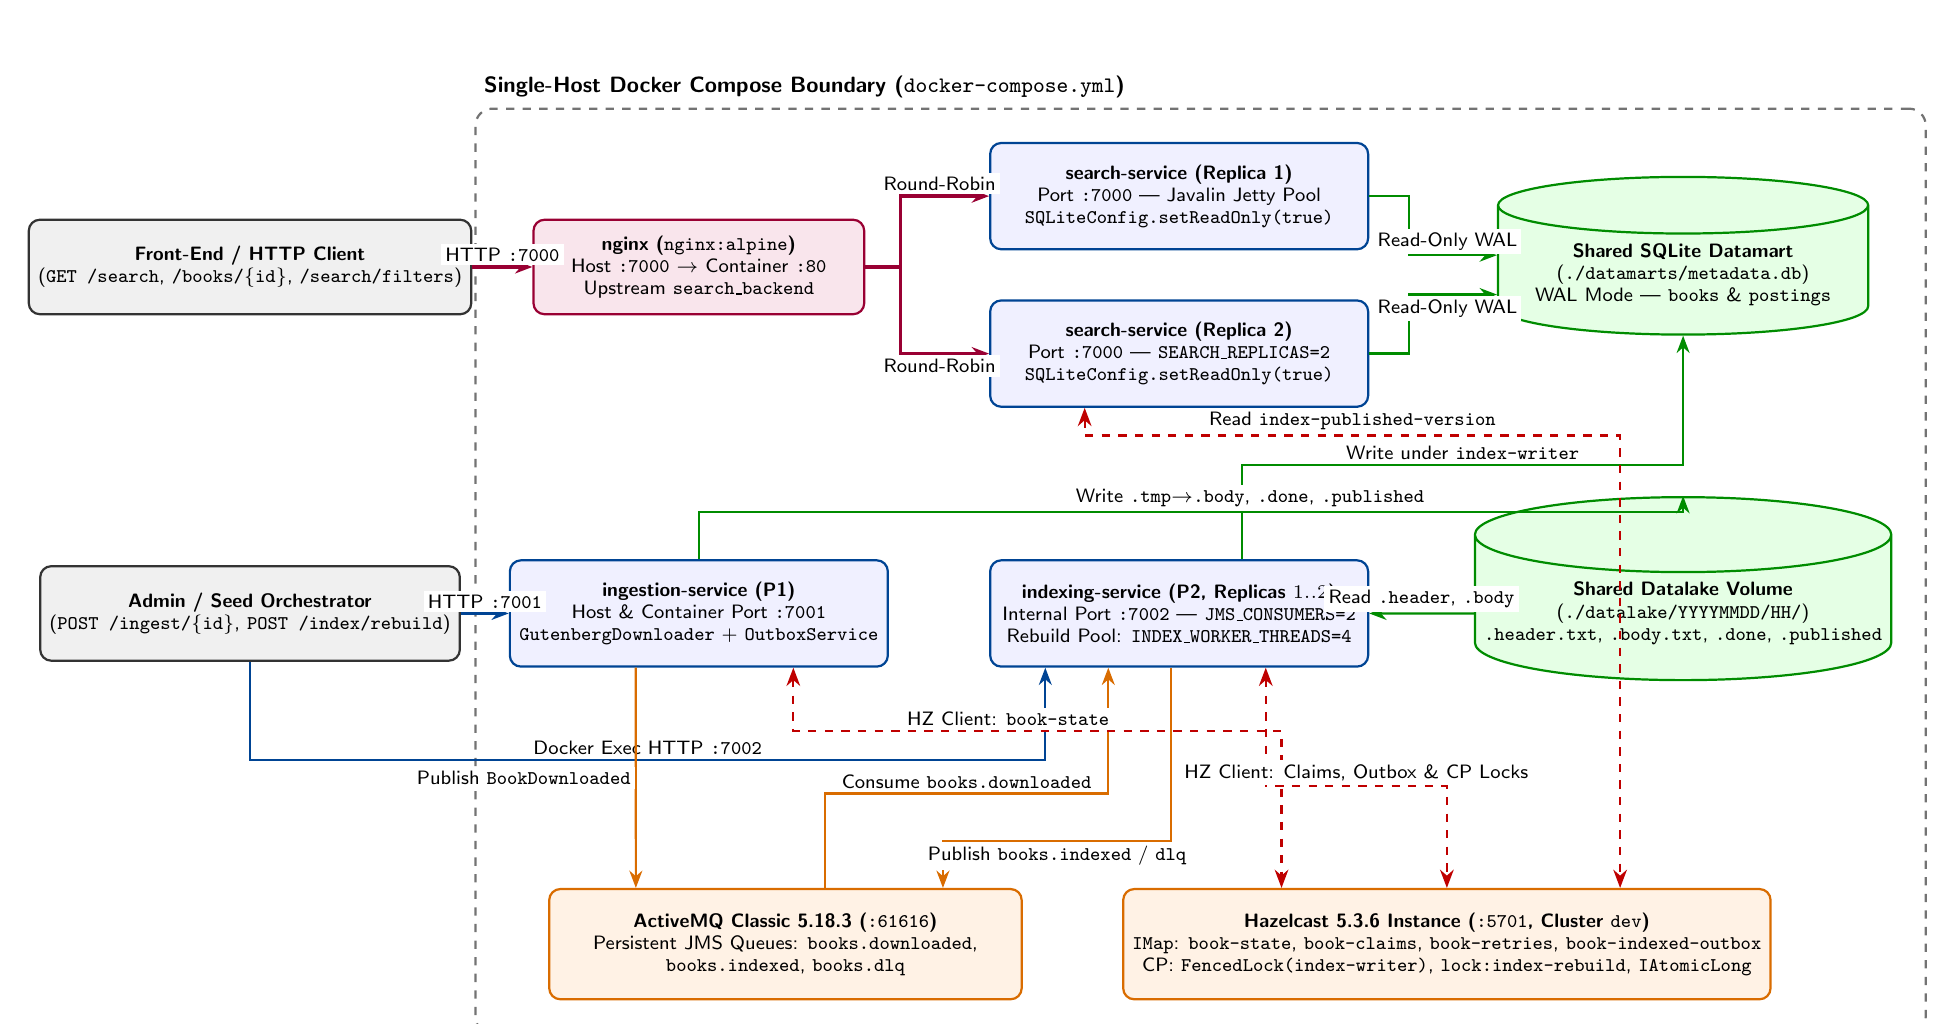
\begin{tikzpicture}[
    boundary/.style={rectangle, rounded corners=6pt, draw=black!55, dashed, thick, inner sep=12pt},
    client/.style={rectangle, rounded corners=4pt, draw=black!80, thick, fill=gray!12, minimum width=4.4cm, minimum height=1.2cm, align=center, font=\scriptsize\sffamily},
    gateway/.style={rectangle, rounded corners=4pt, draw=purple!80!black, thick, fill=purple!10, minimum width=4.2cm, minimum height=1.2cm, align=center, font=\scriptsize\sffamily},
    service/.style={rectangle, rounded corners=4pt, draw=ulpgcblue, thick, fill=blue!6, minimum width=4.8cm, minimum height=1.35cm, align=center, font=\scriptsize\sffamily},
    infra/.style={rectangle, rounded corners=4pt, draw=orange!85!black, thick, fill=orange!10, minimum width=6.0cm, minimum height=1.4cm, align=center, font=\scriptsize\sffamily},
    storage/.style={cylinder, shape border rotate=90, aspect=0.18, draw=green!55!black, thick, fill=green!10, minimum width=4.7cm, minimum height=1.45cm, align=center, font=\scriptsize\sffamily},
    http_ext/.style={-{Stealth[length=2.2mm]}, very thick, draw=purple!80!black},
    http_int/.style={-{Stealth[length=2.2mm]}, thick, draw=ulpgcblue},
    jms_flow/.style={-{Stealth[length=2.2mm]}, thick, draw=orange!85!black},
    hz_flow/.style={<->, >=Stealth, thick, dashed, draw=red!75!black},
    io_flow/.style={-{Stealth[length=2.2mm]}, thick, draw=green!55!black},
    lbl/.style={font=\scriptsize\sffamily, fill=white, inner sep=1.5pt}
]

% Column 1: External & Operational Clients (x = 0)
\node[client] (fe_client) at (0, 4.4) {\textbf{Front-End / HTTP Client}\\(\texttt{GET /search}, \texttt{/books/\{id\}}, \texttt{/search/filters})};
\node[client] (admin_client) at (0, 0.0) {\textbf{Admin / Seed Orchestrator}\\(\texttt{POST /ingest/\{id\}}, \texttt{POST /index/rebuild})};

% Column 2: Gateway & Ingestion (x = 5.7)
\node[gateway] (nginx) at (5.7, 4.4) {\textbf{nginx (\texttt{nginx:alpine})}\\Host \texttt{:7000} $\to$ Container \texttt{:80}\\Upstream \texttt{search\_backend}};
\node[service] (ingestion) at (5.7, 0.0) {\textbf{ingestion-service (P1)}\\Host \& Container Port \texttt{:7001}\\\texttt{GutenbergDownloader} + \texttt{OutboxService}};

% Column 3: Search Replicas & Indexing Service (x = 11.8)
\node[service] (search1) at (11.8, 5.3) {\textbf{search-service (Replica 1)}\\Port \texttt{:7000} | Javalin Jetty Pool\\\texttt{SQLiteConfig.setReadOnly(true)}};
\node[service] (search2) at (11.8, 3.3) {\textbf{search-service (Replica 2)}\\Port \texttt{:7000} | \texttt{SEARCH\_REPLICAS=2}\\\texttt{SQLiteConfig.setReadOnly(true)}};
\node[service] (indexing) at (11.8, 0.0) {\textbf{indexing-service (P2, Replicas $1..2$)}\\Internal Port \texttt{:7002} | \texttt{JMS\_CONSUMERS=2}\\Rebuild Pool: \texttt{INDEX\_WORKER\_THREADS=4}};

% Column 4: Shared Storage Volumes (x = 18.2)
\node[storage] (datamart) at (18.2, 4.3) {\textbf{Shared SQLite Datamart}\\(\texttt{./datamarts/metadata.db})\\WAL Mode | \texttt{books} \& \texttt{postings}};
\node[storage] (datalake) at (18.2, 0.0) {\textbf{Shared Datalake Volume}\\(\texttt{./datalake/YYYYMMDD/HH/})\\\texttt{.header.txt}, \texttt{.body.txt}, \texttt{.done}, \texttt{.published}};

% Bottom Row: ActiveMQ & Hazelcast (y = -4.2)
\node[infra] (activemq) at (6.8, -4.2) {\textbf{ActiveMQ Classic 5.18.3 (\texttt{:61616})}\\Persistent JMS Queues: \texttt{books.downloaded},\\\texttt{books.indexed}, \texttt{books.dlq}};
\node[infra] (hazelcast) at (15.2, -4.2) {\textbf{Hazelcast 5.3.6 Instance (\texttt{:5701}, Cluster \texttt{dev})}\\\texttt{IMap}: \texttt{book-state}, \texttt{book-claims}, \texttt{book-retries}, \texttt{book-indexed-outbox}\\CP: \texttt{FencedLock(index-writer)}, \texttt{lock:index-rebuild}, \texttt{IAtomicLong}};

% Single-Host Docker Boundary
\begin{scope}[on background layer]
    \node[boundary, fit=(nginx) (search1) (search2) (ingestion) (indexing) (datamart) (datalake) (activemq) (hazelcast), label={[font=\footnotesize\bfseries\sffamily, anchor=south west]north west:Single-Host Docker Compose Boundary (\texttt{docker-compose.yml})}] (host_box) {};
\end{scope}

% 1. Front-End HTTP Routing
\draw[http_ext] (fe_client.east) -- node[lbl, above] {HTTP \texttt{:7000}} (nginx.west);
\draw[http_ext] (nginx.east) -- ++(0.45,0) |- node[lbl, pos=0.72, above] {Round-Robin} (search1.west);
\draw[http_ext] (nginx.east) -- ++(0.45,0) |- node[lbl, pos=0.72, below] {Round-Robin} (search2.west);

% 2. Internal & Operational HTTP
\draw[http_int] (admin_client.east) -- node[lbl, above] {HTTP \texttt{:7001}} (ingestion.west);
\draw[http_int] (admin_client.south) -- ++(0,-1.25) -| node[lbl, pos=0.25, above] {Docker Exec HTTP \texttt{:7002}} ([xshift=-1.7cm]indexing.south);

% 3. Storage I/O Paths (Separated Horizontal Lanes at y = 1.9 and y = 1.25)
\draw[io_flow] (search1.east) -- ++(0.5,0) |- node[lbl, pos=0.72, above] {Read-Only WAL} ([yshift=0.25cm]datamart.west);
\draw[io_flow] (search2.east) -- ++(0.5,0) |- node[lbl, pos=0.72, below] {Read-Only WAL} ([yshift=-0.25cm]datamart.west);
\draw[io_flow] ([xshift=0.8cm]indexing.north) -- ++(0,1.2) -| node[lbl, pos=0.25, above] {Write under \texttt{index-writer}} (datamart.south);
\draw[io_flow] (ingestion.north) -- ++(0,0.6) -| node[lbl, pos=0.28, above] {Write \texttt{.tmp}$\to$\texttt{.body}, \texttt{.done}, \texttt{.published}} (datalake.north);
\draw[io_flow] (datalake.west) -- node[lbl, above] {Read \texttt{.header}, \texttt{.body}} (indexing.east);

% 4. ActiveMQ JMS Messaging (Separated Lanes at y = -2.2 and y = -3.0)
\draw[jms_flow] ([xshift=-0.8cm]ingestion.south) -- node[lbl, left] {Publish \texttt{BookDownloaded}} ([xshift=-1.9cm]activemq.north);
\draw[jms_flow] ([xshift=0.5cm]activemq.north) -- ++(0,1.2) -| node[lbl, pos=0.25, above] {Consume \texttt{books.downloaded}} ([xshift=-0.9cm]indexing.south);
\draw[jms_flow] ([xshift=-0.1cm]indexing.south) -- ++(0,-2.2) -| node[lbl, pos=0.25, below] {Publish \texttt{books.indexed} / \texttt{dlq}} ([xshift=2.0cm]activemq.north);

% 5. Hazelcast Client-to-Instance Coordination
\draw[hz_flow] ([xshift=1.2cm]ingestion.south) -- ++(0,-0.8) -| node[lbl, pos=0.22, above] {HZ Client: \texttt{book-state}} ([xshift=-2.1cm]hazelcast.north);
\draw[hz_flow] ([xshift=1.1cm]indexing.south) -- ++(0,-1.5) -| node[lbl, pos=0.25, above] {HZ Client: Claims, Outbox \& CP Locks} (hazelcast.north);
\draw[hz_flow] ([xshift=-1.2cm]search2.south) -- ++(0,-0.35) -| node[lbl, pos=0.25, above] {Read \texttt{index-published-version}} ([xshift=2.2cm]hazelcast.north);

\end{tikzpicture}%
}
\caption{Stage 2 Service-Oriented Architecture (SOA) showing external Front-End HTTP routing, internal/operational HTTP endpoints, ActiveMQ JMS queues, Hazelcast Client-to-Instance coordination structures, and shared volumes within the single-host Docker Compose boundary.}
\label{fig:soa_architecture}
\end{figure}

\subsection{Container Inventory, Resource Limits, and Concurrency Hierarchy}
Table~\ref{tab:container_inventory} details the six services configured in \path{docker-compose.yml} and \path{.env.example}, including their base images, port mappings, JVM heap flags (\texttt{-Xmx}), Docker cgroup CPU/RAM limits, and default replica counts.

\begin{table}[!htbp]
\centering
\caption{Stage 2 Docker Compose service inventory, port mappings, JVM flags, and cgroup resource limits.}
\label{tab:container_inventory}
\scriptsize
\setlength{\tabcolsep}{3.5pt}
\renewcommand{\arraystretch}{1.2}
\begin{tabularx}{\textwidth}{L{1.4cm} L{3.2cm} C{0.9cm} C{0.9cm} C{2.3cm} L{2.5cm} Y}
\toprule
\textbf{Service} & \textbf{Base Image / Runtime} & \textbf{Host} & \textbf{Int.} & \textbf{Replicas} & \textbf{CPU / RAM / Heap} & \textbf{Primary Responsibility} \\
\midrule
\texttt{nginx} & \texttt{nginx:alpine} & \texttt{7000} & \texttt{80} & $1$ & \texttt{0.5} CPU / \texttt{128M} / N/A & Reverse proxy (\texttt{worker\_connections 1024}) load-balancing \texttt{search:7000}. \\
\texttt{search} & \texttt{eclipse-temurin:17-jre-jammy} & None & \texttt{7000} & $2$ (\texttt{SEARCH\_REPLICAS}) & \texttt{1.0} CPU / \texttt{768M} / \texttt{-Xmx512m} & Stateless read-only SQLite WAL query engine and Hazelcast client version reader. \\
\texttt{ingestion} & \texttt{eclipse-temurin:17-jre-jammy} & \texttt{7001} & \texttt{7001} & $1$ & \texttt{1.0} CPU / \texttt{768M} / \texttt{-Xmx512m} & Gutenberg downloader, atomic datalake storage, and \texttt{OutboxService} publisher. \\
\texttt{indexing} & \texttt{eclipse-temurin:17-jre-jammy} & None & \texttt{7002} & $1..2$ (\texttt{INDEXING\_REPLICAS}) & \texttt{1.5} CPU / \texttt{1024M} / \texttt{-Xmx512m} & Multi-consumer JMS indexer (\texttt{JMS\_CONSUMERS=2}), \texttt{IndexRebuilder} (\texttt{INDEX\_WORKER\_THREADS=4}). \\
\texttt{activemq} & \texttt{apache/activemq-classic:5.18.3} & \texttt{61616} & \texttt{61616} & $1$ & \texttt{1.0} CPU / \texttt{512M} / \texttt{-Xmx256m} & Persistent OpenWire JMS broker (KahaDB store in \texttt{./activemq-data}). \\
\texttt{hazelcast} & \texttt{hazelcast/hazelcast:5.3.6} & \texttt{5701} & \texttt{5701} & $1$ & \texttt{1.0} CPU / \texttt{512M} / Default & Stateful Hazelcast cluster \textbf{Instance} (\texttt{hazelcast/hazelcast.yaml}, cluster \texttt{dev}). \\
\bottomrule
\end{tabularx}
\end{table}

% ==============================================================================
% SECTION 3: API DESIGN AND CONTRACTS
% ==============================================================================
\section{API Design and Contracts}
\label{sec:api_contracts}

All synchronous HTTP interfaces and asynchronous non-HTTP coordination protocols are formally documented in \path{docs/openapi.yaml} (OpenAPI 3.0.3~\cite{openapi_spec}). In accordance with SOA design principles, we separate \textbf{Front-End-Facing APIs} from \textbf{Internal \& Operational Service APIs}.

\subsection{Front-End-Facing HTTP API (\texttt{search-service} via Nginx on Port \texttt{7000})}
Table~\ref{tab:frontend_api} inventories the public read-only endpoints exposed to end-user applications through the Nginx reverse proxy (\texttt{http://localhost:7000}).

\begin{table}[!htbp]
\centering
\caption{Front-End-Facing HTTP API exposed by \texttt{search-service} behind Nginx (\texttt{http://localhost:7000}).}
\label{tab:frontend_api}
\scriptsize
\setlength{\tabcolsep}{4pt}
\renewcommand{\arraystretch}{1.2}
\begin{tabularx}{\textwidth}{L{2.5cm} L{3.6cm} L{1.9cm} Y}
\toprule
\textbf{Method \& Path} & \textbf{Query / Path Parameters} & \textbf{Status Codes} & \textbf{Contract, Ranking, Pagination, and Error Semantics} \\
\midrule
\texttt{GET /search} & \texttt{q} (req., string); \texttt{author} (opt., substring); \texttt{language} (opt., ISO-639-1); \texttt{year} (opt., $1000..9999$); \texttt{offset} (opt., $\ge 0$, def.\ $0$); \texttt{limit} (opt., $1..100$, def.\ $20$) & \texttt{200 OK}, \texttt{400 Bad Req.}, \texttt{500 Int.\ Err.} & Single-term full-text search. Extracts the first token matching \texttt{\textbackslash b[a-z]\{3,\}\textbackslash b}. Stop words or $<3$-letter queries return \texttt{200 OK} with \texttt{total: 0, results: []}. Ranked deterministically by \texttt{p.freq DESC, b.book\_id ASC}. \texttt{total} reports the unpaginated global match count via SQL \texttt{COUNT(*) OVER()}, whereas \texttt{results.size()} is bounded by \texttt{limit} ($\le 100$). \\
\addlinespace[2pt]
\texttt{GET /books/\{id\}} & \texttt{id} (req.\ path integer) & \texttt{200 OK}, \texttt{400 Bad Req.}, \texttt{404 Not Found}, \texttt{500 Int.\ Err.} & Returns book metadata JSON: \texttt{\{book\_id, title, author, language, year\}}, where \texttt{language} and \texttt{year} are nullable. Non-integer \texttt{id} returns \texttt{400}; absent \texttt{book\_id} returns \texttt{404}. \\
\addlinespace[2pt]
\texttt{GET /search/filters} & None & \texttt{200 OK}, \texttt{500 Int.\ Err.} & Returns sorted distinct non-null filter domains currently indexed in SQLite: \texttt{\{"languages": ["en","es","fr"], "years": [1975,...,2008]\}}. \\
\bottomrule
\end{tabularx}
\end{table}

\paragraph{Strict Distinction Between \texttt{200 OK} (Empty), \texttt{400 Bad Request}, \texttt{404 Not Found}, and \texttt{500 Internal Server Error}:}
\begin{itemize}[leftmargin=*,nosep]
    \item \textbf{\texttt{200 OK} with Empty Results:} Returned when \texttt{q} is syntactically valid (non-blank) and all filter parameters are valid, even if zero documents match, \texttt{q} is a stop word (e.g., \texttt{q=the}), or \texttt{q} contains no token of length $\ge 3$ (e.g., \texttt{q=hi}).
    \item \textbf{\texttt{400 Bad Request}:} Returned with \texttt{\{"error": "Bad Request", "message": "..."\}} when \texttt{q} is missing or blank, \texttt{offset < 0} or non-integer, \texttt{limit < 1} or \texttt{limit > 100} or non-integer, \texttt{year} $\notin [1000, 9999]$ or non-integer, \texttt{language} is not in the 12-code ISO-639-1 whitelist (\texttt{en, es, fr, de, it, pt, la, nl, ru, zh, ja, el}), or \texttt{\{id\}} in \texttt{/books/\{id\}} is non-numeric.
    \item \textbf{\texttt{500 Internal Server Error}:} Handled centrally by \texttt{ApiErrors.internalServerError(ctx, gson)}, which logs the exception server-side via SLF4J and returns strictly \texttt{\{"error": "Internal server error"\}}, preventing any leakage of SQLite paths, table names, or stack traces.
\end{itemize}

\subsection{Internal and Operational Service HTTP APIs}
Table~\ref{tab:internal_api} catalogs the internal control-plane and operational endpoints exposed by \texttt{ingestion-service} (\texttt{:7001}), \texttt{indexing-service} (\texttt{:7002}), and \texttt{search-service} (\texttt{:7000}).

\begin{table}[!htbp]
\centering
\caption{Internal and operational HTTP endpoints across \texttt{ingestion-service}, \texttt{indexing-service}, and \texttt{search-service}.}
\label{tab:internal_api}
\scriptsize
\setlength{\tabcolsep}{3.5pt}
\renewcommand{\arraystretch}{1.16}
\begin{tabularx}{\textwidth}{L{2.1cm} L{3.2cm} L{1.5cm} L{1.8cm} Y}
\toprule
\textbf{Service} & \textbf{Method \& Path} & \textbf{Layer} & \textbf{Codes} & \textbf{Completion \& Idempotency Contract} \\
\midrule
\texttt{ingestion} (\texttt{:7001}) & \texttt{POST /ingest/\{id\}} & Internal & \texttt{200, 400, 404, 500} & Synchronously downloads book \texttt{id} from Gutenberg, writes \texttt{.header.txt}, \texttt{.body.txt}, and \texttt{.done}, and triggers \texttt{OutboxService.publishBook()} (\texttt{status: "downloaded"}). If \texttt{.done} already exists, skips download and returns \texttt{200 OK} (\texttt{"already\_downloaded"}), re-running outbox publication if \texttt{.published} is missing. Returns \texttt{404} (\texttt{FAILED\_404}) if absent on Gutenberg. \\
\texttt{ingestion} (\texttt{:7001}) & \texttt{GET /ingest/status/\{id\}} & Internal & \texttt{200, 400} & Checks whether \texttt{<id>.done} exists in \texttt{./datalake}; returns \texttt{\{book\_id, status: "available" | "not\_found"\}}. \\
\texttt{ingestion} (\texttt{:7001}) & \texttt{GET /ingest/list} & Operational & \texttt{200} & Walks \texttt{./datalake} (depth $\le 4$) for \texttt{*.done} files and returns \texttt{\{count, books: [id1, ...]\}}. \\
\texttt{ingestion} (\texttt{:7001}) & \texttt{GET /status} & Operational & \texttt{200} & Returns \texttt{\{"service": "ingestion-service", "status": "running"\}}. \\
\midrule
\texttt{indexing} (\texttt{:7002}) & \texttt{POST /index/update/\{id\}} & Internal & \texttt{200, 400, 404, 500} & Synchronously parses book \texttt{id} from \texttt{./datalake} and updates SQLite under \texttt{FencedLock("index-writer")} (\texttt{force=true}). Returns \texttt{404} if no \texttt{.done} marker exists. \\
\texttt{indexing} (\texttt{:7002}) & \texttt{POST /index/rebuild} & Operational & \texttt{200, 409, 500} & Builds replacement index in \texttt{metadata.db.rebuild-<uuid>.tmp} under \texttt{lock:index-rebuild} and swaps rows atomically under \texttt{index-writer}. Returns \texttt{\{books\_processed, elapsed\_time\}}. Concurrent calls fail fast with \texttt{409 Conflict}. \\
\texttt{indexing} (\texttt{:7002}) & \texttt{GET /index/status} & Operational & \texttt{200} & Returns \texttt{\{books\_indexed, last\_update, index\_size\_MB\}} from SQLite \texttt{books} count and file byte length. \\
\texttt{indexing} (\texttt{:7002}) & \texttt{GET /status} & Operational & \texttt{200} & Returns \texttt{\{"service": "indexing-service", "status": "running"\}}. \\
\midrule
\texttt{search} (\texttt{:7000}) & \texttt{GET /status} & Operational & \texttt{200} & Reports \texttt{service}, \texttt{status} (\texttt{"running"} or \texttt{"degraded"}), \texttt{hazelcast\_status} (\texttt{"connected"} / \texttt{"disconnected"}), \texttt{sqlite\_status} (\texttt{"read-only-connected"} / \texttt{"error"} via \texttt{SELECT 1}), and \texttt{active\_index\_version}. \\
\bottomrule
\end{tabularx}
\end{table}

\subsection{Non-HTTP Asynchronous Messaging and Distributed Coordination Contracts}
Table~\ref{tab:non_http_contracts} specifies all asynchronous queues in ActiveMQ Classic 5.18.3, filesystem state markers in \path{./datalake}, and distributed coordination structures in Hazelcast 5.3.6 defined in \path{SystemConstants.java} and \path{docs/openapi.yaml}.

\begin{table}[!htbp]
\centering
\caption{Non-HTTP event queues, filesystem markers, and Hazelcast distributed coordination contracts.}
\label{tab:non_http_contracts}
\scriptsize
\setlength{\tabcolsep}{3.5pt}
\renewcommand{\arraystretch}{1.15}
\begin{tabularx}{\textwidth}{L{2.1cm} L{3.1cm} L{2.8cm} Y}
\toprule
\textbf{Subsystem} & \textbf{Identifier} & \textbf{Type / Primitive} & \textbf{Schema, Producer/Consumer, and Consistency Protocol} \\
\midrule
Datalake FS & \texttt{<id>.done}, \texttt{<id>.published} & Filesystem Markers & \texttt{<id>.done} (\texttt{"READY"}, $5\text{ B}$) is written after \texttt{<id>.header.txt} and \texttt{<id>.tmp} $\to$ \texttt{<id>.body.txt} (\texttt{ATOMIC\_MOVE}). \texttt{<id>.published} (\texttt{"PUBLISHED"}, $9\text{ B}$) is written after ActiveMQ accepts \texttt{BookDownloaded}. \\
ActiveMQ 5.18.3 & \texttt{books.downloaded} & JMS Queue (\texttt{PERSISTENT}) & Producer: \texttt{OutboxService} (\texttt{AUTO\_ACKNOWLEDGE}). Consumer: \texttt{BookDownloadedConsumer} (\texttt{CLIENT\_ACKNOWLEDGE}). Payload (\texttt{BookDownloaded}): \texttt{\{"event\_id": "<uuid>", "book\_id": 1342, "path": "...", "downloaded\_at": "<ISO-8601>"\}}. \\
ActiveMQ 5.18.3 & \texttt{books.indexed} & JMS Queue (\texttt{PERSISTENT}) & Producer: \texttt{BookIndexedPublisher} (backed by Hazelcast \texttt{book-indexed-outbox}). Payload (\texttt{BookIndexed}): \texttt{\{"event\_id": "<uuid>", "book\_id": 1342, "index\_version": 25, "indexed\_at": "<ISO-8601>"\}}. \\
ActiveMQ 5.18.3 & \texttt{books.dlq} & Dead-Letter Queue & Producer: \texttt{BookDownloadedConsumer} when \texttt{book-retries} reaches \texttt{MAX\_RETRIES} (default $3$). Payload: \texttt{\{"book\_id": 1342, "error": "...", "attempts": 3\}}. \\
Hazelcast AP & \texttt{book-state} & \texttt{IMap<Integer, String>} & Tracks book lifecycle: \texttt{DOWNLOADED} $\to$ \texttt{INDEXING} $\to$ \texttt{INDEXED} (or \texttt{FAILED}). State transitions during JMS consumption are guarded by per-key lock \texttt{bookState.lock(bookId)}. \\
Hazelcast AP & \texttt{book-claims} & \texttt{IMap<Integer, BookClaim>} & Stores \texttt{BookClaim(String claimantId, long claimedAtMs)}. Active claims younger than \texttt{INDEXING\_TIMEOUT\_MS} ($300,000\text{ ms}$) yield \texttt{RETRY\_LATER}; expired claims are taken over. \\
Hazelcast AP & \texttt{book-retries} & \texttt{IMap<Integer, Integer>} & Tracks consecutive indexing exceptions per \texttt{book\_id}. Removed upon \texttt{INDEXED} or \texttt{ALREADY\_INDEXED}. \\
Hazelcast AP & \texttt{book-indexed-outbox} & \texttt{IMap<String, String>} & Keyed by \texttt{event\_id}, stores JSON \texttt{BookIndexed} payloads recorded under \texttt{LOCK\_INDEX\_WRITER} until \texttt{BookIndexedPublisher} confirms JMS delivery. \\
Hazelcast CP & \texttt{index-writer} & \texttt{FencedLock} & Serializes all SQLite write transactions (\texttt{saveBookIndex} and \texttt{replaceContentsFrom}), \texttt{index-published-version} increments, and \texttt{book-indexed-outbox} recording. \\
Hazelcast CP & \texttt{lock:index-rebuild} & \texttt{FencedLock} & Acquired via non-blocking \texttt{tryLock()} by \texttt{IndexRebuilder} to guarantee at most one active rebuild across all replicas (\texttt{409 Conflict} on contention). \\
Hazelcast CP & \texttt{index-published-version} & \texttt{IAtomicLong} & Monotonically increasing index generation counter incremented on each book commit and full rebuild; exposed by \texttt{search-service} on \texttt{GET /status}. \\
\bottomrule
\end{tabularx}
\end{table}

\subsection{Functional, End-to-End, and Resilience Validation Suite}
Contract compliance is verified through three complementary validation suites:
\begin{enumerate}[leftmargin=*,nosep]
    \item \textbf{Interactive HTTP Contract Suite (\path{tests/search-api-tests.http}):} Contains \textbf{22 HTTP test requests} covering health checks (\texttt{\#1}), filter discovery (\texttt{\#2}), single and combined filters (\texttt{\#3--\#7}), pagination (\texttt{\#8--\#9}), empty matches and stop words returning \texttt{200 OK} (\texttt{\#10--\#11}), nine negative \texttt{400 Bad Request} boundary checks (\texttt{\#12--\#20}: missing \texttt{q}, \texttt{limit=-1}, \texttt{limit=200}, \texttt{limit=abc}, \texttt{year=abc}, \texttt{year=999}, \texttt{offset=-5}, \texttt{offset=xyz}, \texttt{language=klingon}), and \texttt{GET /books/\{id\}} \texttt{200}/\texttt{404} checks (\texttt{\#21--\#22}).
    \item \textbf{Automated End-to-End Validation Scripts (\path{scripts/test_end_to_end.ps1} and \texttt{.sh}):} Executed via \texttt{powershell -NoProfile -ExecutionPolicy Bypass -File ".\textbackslash scripts\textbackslash test\_end\_to\_end.ps1"}. The script verifies container readiness across ports \texttt{7000} and \texttt{7001} plus the running \texttt{indexing} container, invokes \path{seed/download_seed.ps1} to ingest all 25 seed books idempotently, polls \texttt{/search} until English (\texttt{q=adventure\&language=en}), Spanish (\texttt{q=quijote\&language=es}), and French (\texttt{q=candide\&language=fr}) books are searchable, and executes \textbf{9 automated assertions} (\textbf{9/9 passed}).
    \item \textbf{Automated Maven Unit \& Integration Test Suite (\texttt{mvn clean test}):} Executes \textbf{41 JUnit 5 tests} across the reactor using embedded ActiveMQ (\texttt{vm://}) brokers, local Hazelcast instances, and isolated \texttt{@TempDir} SQLite databases (detailed in Section~\ref{subsec:resilience_tests}).
\end{enumerate}

% ==============================================================================
% SECTION 4: MICROSERVICE IMPLEMENTATION
% ==============================================================================
\section{Microservice Implementation}
\label{sec:implementation}

The repository is organized as a multi-module Maven reactor (\path{pom.xml}, group \texttt{com.fourbytees}, artifact \texttt{stage\_2}, version \texttt{1.0.0}) managing centralized dependency versions: Javalin \texttt{6.1.3}, Gson \texttt{2.11.0}, Hazelcast \texttt{5.3.6}, ActiveMQ \texttt{5.18.3}, Xerial SQLite JDBC \texttt{3.45.1.0}, SLF4J \texttt{2.0.9}, JUnit Jupiter \texttt{5.10.2}, and OpenJDK JMH \texttt{1.37}.

\subsection{Code Hygiene and Benchmark Isolation (Addressing Stage 1 Feedback \#41)}
To maintain strict separation between production code and experimental harnesses:
\begin{itemize}[leftmargin=*,nosep]
    \item All JMH microbenchmark classes---\texttt{IndexingMicroBenchmark.java} (in \texttt{indexing-service}) and \texttt{SearchMicroBenchmark.java} (in \texttt{search-service})---reside exclusively under \path{src/test/java/com/fourbytees/benchmark/}.
    \item In the root \path{pom.xml}, \texttt{jmh-core}, \texttt{jmh-generator-annprocess}, \texttt{junit-jupiter}, and \texttt{activemq-broker} are declared strictly with \texttt{<scope>test</scope>}. Consequently, the production shaded JARs built by \texttt{maven-shade-plugin} in the multi-stage Dockerfiles (\texttt{mvn -pl <service> -am clean package -DskipTests}) contain zero benchmark or test classes.
    \item Build-time \path{dependency-reduced-pom.xml} files are suppressed via \texttt{createDependencyReducedPom=false} in \path{pom.xml} and ignored in \path{.gitignore}, ensuring a clean working tree.
\end{itemize}

\subsection{Shared Module (\texttt{common-dto})}
\texttt{common-dto} encapsulates cross-service constants and wire contracts:
\begin{itemize}[leftmargin=*,nosep]
    \item \texttt{SystemConstants}: Defines the canonical state names (\texttt{DOWNLOADED}, \texttt{INDEXING}, \texttt{INDEXED}, \texttt{FAILED}), Hazelcast map names (\texttt{book-state}, \texttt{book-claims}, \texttt{book-retries}), CP lock/atomic names (\texttt{index-writer}, \texttt{index-published-version}), and ActiveMQ queue names (\texttt{books.downloaded}, \texttt{books.indexed}, \texttt{books.dlq}).
    \item \texttt{BookDownloaded} and \texttt{BookIndexed}: Serializable DTOs with snake\_case JSON fields (\texttt{event\_id}, \texttt{book\_id}, \texttt{path}, \texttt{downloaded\_at} and \texttt{event\_id}, \texttt{book\_id}, \texttt{index\_version}, \texttt{indexed\_at}).
    \item \texttt{HazelcastClientFactory} and \texttt{JmsClientFactory}: Instantiate lightweight \texttt{HazelcastClient} connections (\texttt{HazelcastClient.newHazelcastClient(clientConfig)}) targeting the cluster member at \texttt{HAZELCAST\_HOST:5701} with a $60\text{ s}$ connect timeout (\texttt{setClusterConnectTimeoutMillis(60000)}) and OpenWire JMS connections.
\end{itemize}

\subsection{Ingestion Service (\texttt{ingestion-service})}
Implemented in package \texttt{com.fourbytees.ingestion} (\texttt{App}, \texttt{IngestionController}, \texttt{GutenbergDownloader}, \texttt{DatalakeStorage}, \texttt{OutboxService}):
\begin{enumerate}[leftmargin=*,nosep]
    \item \textbf{Gutenberg Acquisition \& Header/Body Splitting (\texttt{GutenbergDownloader}):} Fetches \path{https://www.gutenberg.org/cache/epub/{id}/pg{id}.txt} using Java 11+ \texttt{HttpClient} ($10\text{ s}$ connect timeout, $15\text{ s}$ request timeout, normal redirect following) with up to $3$ attempts and linear backoff ($1\text{ s}, 2\text{ s}$). If Gutenberg returns HTTP \texttt{404}, it throws \texttt{RuntimeException("FAILED\_404")}, which \texttt{IngestionController} maps to HTTP \texttt{404}. On HTTP \texttt{200}, \texttt{splitHeaderAndBody()} locates the line containing \texttt{"*** START OF"}, extracting everything before it as \texttt{header} and everything after the marker line as \texttt{body}.
    \item \textbf{Atomic Datalake Persistence (\texttt{DatalakeStorage}):} Partitions files by ingestion date and hour (\path{datalake/<yyyyMMdd>/<HH>/}). To prevent \texttt{indexing-service} from ever reading a half-written book body, \texttt{saveBook()} writes \texttt{<id>.header.txt}, writes the body to a temporary file \texttt{<id>.tmp}, atomically renames \texttt{<id>.tmp} $\to$ \texttt{<id>.body.txt} via \texttt{Files.move(..., REPLACE\_EXISTING, ATOMIC\_MOVE)}, and finally creates the completion marker \texttt{<id>.done} containing \texttt{"READY"}.
    \item \textbf{Crash-Consistent Transactional Outbox (\texttt{OutboxService}):} Only after \texttt{<id>.done} is durable on disk does \texttt{OutboxService.publishBook(bookId, path)} execute the three-step publication protocol: (i) put \texttt{STATE\_DOWNLOADED} into Hazelcast \texttt{IMap("book-state")}, (ii) send a \texttt{DeliveryMode.PERSISTENT} JSON \texttt{BookDownloaded} message to ActiveMQ queue \texttt{books.downloaded}, and (iii) create \texttt{<id>.published} (\texttt{"PUBLISHED"}) on disk. At service startup (\texttt{App.main}), \texttt{outboxService.runOutboxCheck()} scans all \texttt{*.done} files in \path{./datalake} and automatically republishes any book lacking a corresponding \texttt{<id>.published} marker.
\end{enumerate}

\subsection{Indexing Service (\texttt{indexing-service})}
Implemented in package \texttt{com.fourbytees.indexing} (\texttt{App}, \texttt{IndexingConfig}, \texttt{IndexingController}, \texttt{BookDownloadedConsumer}, \texttt{JmsClientFactory}, \texttt{HeaderParser}, \texttt{BodyTokenizer}, \texttt{SqliteRepository}, \texttt{BookClaim}, \texttt{BookIndexedPublisher}, \texttt{IndexingOrchestrator}, \texttt{IndexRebuilder}):
\begin{enumerate}[leftmargin=*,nosep]
    \item \textbf{Header Metadata Extraction (\texttt{HeaderParser}):} Streams \texttt{<id>.header.txt} line-by-line in UTF-8, supporting multiline indented continuation lines for \texttt{Title:} and \texttt{Author:}, extracting the 4-digit release/posting year via \texttt{\textbackslash b(1\textbackslash d\{3\}|20\textbackslash d\{2\})\textbackslash b} from \texttt{Release date:} or \texttt{Posting date:} lines, and normalizing the primary \texttt{Language:} name into a 12-language ISO-639-1 code (\texttt{english}$\to$\texttt{en}, \texttt{spanish}$\to$\texttt{es}, \texttt{french}$\to$\texttt{fr}, etc., or \texttt{null} if unrecognized).
    \item \textbf{Frozen Stage 1 Tokenization Contract (\texttt{BodyTokenizer}):} Converts \texttt{<id>.body.txt} to lowercase and extracts tokens matching \texttt{\textbackslash b[a-z]\{3,\}\textbackslash b}. Every regex match increments the 0-based \texttt{wordIndex} counter \emph{before} checking the 30-word \texttt{STOP\_WORDS} set (\texttt{a, an, and, are, as, at, be, but, by, for, if, in, into, is, it, no, not, of, on, or, such, that, the, their, then, there, these, they, this, to}), ensuring positional postings \texttt{Map<String, List<Integer>>} preserve exact word positions without renumbering.
    \item \textbf{Lease-Based Claim Coordination (\texttt{IndexingOrchestrator} \& \texttt{BookClaim}):} When \texttt{BookDownloadedConsumer} receives a message from \texttt{books.downloaded}, \texttt{claimBook(bookId, bookState, bookClaims)} acquires the key-level Hazelcast lock \texttt{bookState.lock(bookId)} and evaluates the state machine:
    \begin{itemize}[nosep]
        \item If \texttt{currentState == INDEXED}, returns \texttt{IndexingResult.ALREADY\_INDEXED} (duplicate message acknowledged immediately).
        \item If \texttt{currentState == DOWNLOADED}, transitions \texttt{book-state} to \texttt{INDEXING}, writes \texttt{new BookClaim(claimantId, now)} to \texttt{book-claims}, and proceeds to parse and index.
        \item If \texttt{currentState == INDEXING}, inspects the existing \texttt{BookClaim}: if \texttt{now - claimedAtMs < INDEXING\_TIMEOUT\_MS} ($300,000\text{ ms}$), returns \texttt{RETRY\_LATER}; if the claim has expired ($\ge 300,000\text{ ms}$), takes over the stale claim with a fresh timestamp and proceeds.
    \end{itemize}
    \item \textbf{Transactional SQLite Persistence \& Post-Commit Outbox (\texttt{SqliteRepository} \& \texttt{BookIndexedPublisher}):} Parsing (\texttt{parseBook}) runs \emph{outside} the global write lock so multiple threads/replicas tokenize in parallel. Once parsed, \texttt{processBook()} acquires \texttt{FencedLock("index-writer")}:
\begin{lstlisting}[language=Java,caption={Coordinated SQLite commit and post-commit outbox recording in \texttt{IndexingOrchestrator.java}.}]
FencedLock lock = hazelcast.getCPSubsystem().getLock(SystemConstants.LOCK_INDEX_WRITER);
lock.lock();
try {
    repository.saveBookIndex(metadata, parsed.postings()); // Single SQLite transaction (DELETE + INSERT)
    newVersion = hazelcast.getCPSubsystem()
            .getAtomicLong(SystemConstants.ATOMIC_INDEX_VERSION)
            .incrementAndGet();
    event = new BookIndexed(UUID.randomUUID().toString(), bookId, newVersion, Instant.now().toString());
    publisher.record(event); // Recorded in Hazelcast IMap("book-indexed-outbox") before unlock
    bookState.put(bookId, SystemConstants.STATE_INDEXED);
    if (bookClaims != null) {
        removeOwnClaim(bookId, bookClaims);
    }
} finally {
    lock.unlock();
}
publisher.publish(event); // Bounded post-commit retries + background outbox relay
\end{lstlisting}
    \item \textbf{Zero-Downtime Atomic Full Rebuild (\texttt{IndexRebuilder}):} Guarded by an in-process \texttt{AtomicBoolean} and distributed \texttt{FencedLock("lock:index-rebuild")} (\texttt{tryLock()}). Builds a complete replacement database at \path{metadata.db.rebuild-<uuid>.tmp} using \texttt{INDEX\_WORKER\_THREADS} ($4$) parallel parser threads in batches of $2 \times \text{workerThreads} = 8$. Once built, it acquires \texttt{FencedLock("index-writer")}, indexes any late-arriving books that became ready during the build, and calls \texttt{repository.replaceContentsFrom(temporaryDb)}, which executes \texttt{ATTACH DATABASE ? AS replacement} and swaps \texttt{main.books} and \texttt{main.postings} inside a single \texttt{BEGIN IMMEDIATE ... COMMIT} transaction followed by \texttt{PRAGMA wal\_checkpoint(PASSIVE)} and cleanup of \texttt{.tmp}, \texttt{-wal}, and \texttt{-shm} side files.
\end{enumerate}

\subsection{Search Service (\texttt{search-service})}
Implemented in package \texttt{com.fourbytees.search} (\texttt{Main}, \texttt{HazelcastConfig}, \texttt{SearchController}, \texttt{BookController}, \texttt{StatusController}, \texttt{ApiErrors}, \texttt{DatabaseManager}):
\begin{itemize}[leftmargin=*,nosep]
    \item \textbf{Read-Only WAL Query Execution (\texttt{DatabaseManager}):} Opens every JDBC connection with \texttt{SQLiteConfig.setReadOnly(true)}. \texttt{searchByTerm()} normalizes \texttt{q} with the frozen Stage 1 regex \texttt{\textbackslash b[a-z]\{3,\}\textbackslash b} and 30-word stop-word filter, then executes a single parameterized query joining \texttt{postings p} and \texttt{books b} with window function \texttt{COUNT(*) OVER() AS total\_matches}, ordered by \texttt{p.freq DESC, b.book\_id ASC} with \texttt{LIMIT ? OFFSET ?}. Because $\text{idf}(t) = \ln(N / \text{df}_t)$ is constant across all documents matching a single query term $t$, ordering by $\text{freq}(t, d)$ descending yields the exact relative single-term TF-IDF ranking.
    \item \textbf{Graceful Degradation (\texttt{HazelcastConfig} \& \texttt{StatusController}):} If Hazelcast is unreachable, \texttt{search-service} continues serving SQLite queries while reporting \texttt{"status": "degraded"}, \texttt{"hazelcast\_status": "disconnected"}, and \texttt{"active\_index\_version": "unknown"} on \texttt{GET /status}.
\end{itemize}

% ==============================================================================
% SECTION 5: DESIGN DECISIONS
% ==============================================================================
\section{Design Decisions}
\label{sec:design_decisions}

\subsection{Hybrid Coordination (ActiveMQ + Hazelcast + Dual Outbox) vs.\ Centralized Orchestration}
A purely centralized orchestrator (where a single controller service synchronously calls ingestion, waits for completion, calls indexing, and updates search replicas via HTTP RPCs) introduces tight temporal coupling and a single point of orchestration failure~\cite{microservices_richardson}. Instead, our hybrid architecture separates \textbf{asynchronous work distribution} (ActiveMQ JMS queues) from \textbf{shared state \& mutual exclusion} (Hazelcast CP/AP primitives):
\begin{itemize}[leftmargin=*,nosep]
    \item \textbf{Temporal Decoupling via Competing Consumers:} \texttt{ingestion-service} returns \texttt{HTTP 200} as soon as the book is sealed in \path{./datalake} with \texttt{<id>.done} and queued in \texttt{books.downloaded}. If \texttt{indexing-service} is temporarily busy with a large novel (e.g., \emph{Moby Dick}), ingestion continues unblocked while ActiveMQ buffers pending events on disk (KahaDB).
    \item \textbf{Elimination of Dual-Write Anomalies via Dual Outbox:} Writing to a filesystem/database and publishing to a message broker is a classic non-atomic dual write~\cite{kleppmann_ddia}. We solve this in both services without heavyweight XA two-phase commit:
    \begin{enumerate}[nosep]
        \item In \texttt{ingestion-service}, \texttt{<id>.done} acts as the durable commit point and \texttt{<id>.published} as the outbox completion marker scanned by \texttt{OutboxService.runOutboxCheck()}.
        \item In \texttt{indexing-service}, \texttt{BookIndexedPublisher.record(event)} writes the serialized \texttt{BookIndexed} event into Hazelcast \texttt{IMap("book-indexed-outbox")} \emph{while still holding} \texttt{FencedLock("index-writer")}. If the broker fails after the SQLite commit, the background thread (\texttt{book-indexed-outbox-relay}, running every \texttt{OUTBOX\_FLUSH\_INTERVAL\_MS = 10,000 ms} for entries older than \texttt{OUTBOX\_MIN\_AGE\_MS = 5,000 ms}) delivers the event later \textbf{without ever repeating the SQLite write}.
    \end{enumerate}
\end{itemize}

\subsection{Three-Tier Concurrency Model: Clients, Container Replicas, and Process Threads}
We explicitly distinguish three orthogonal concurrency dimensions in our architecture:
\begin{enumerate}[leftmargin=*,nosep]
    \item \textbf{HTTP Client Concurrency ($c \in \{1, 4, 8, 16, 32\}$):} Number of simultaneous external HTTP requests arriving at Nginx (\texttt{:7000}). Nginx multiplexes connections asynchronously (\texttt{worker\_connections 1024}) across upstream \texttt{search-service} containers.
    \item \textbf{Container / Process Replicas (\texttt{SEARCH\_REPLICAS=2}, \texttt{INDEXING\_REPLICAS=1..2}):} Separate OS containers with isolated JVM heaps (\texttt{-Xmx512m}). Scaling \texttt{SEARCH\_REPLICAS} increases parallel read capacity across CPU cores; scaling \texttt{INDEXING\_REPLICAS} increases parallel document parsing and JMS consumption across processes.
    \item \textbf{Intra-Process Threads:}
    \begin{itemize}[nosep]
        \item \emph{Javalin/Jetty HTTP Threads:} Handle incoming REST requests inside each microservice.
        \item \emph{JMS Consumer Threads (\texttt{JMS\_CONSUMERS=2}):} Dedicated daemon threads (\texttt{jms-consumer-0}, \texttt{jms-consumer-1}) inside each \texttt{indexing-service} replica pulling messages concurrently from \texttt{books.downloaded}.
        \item \emph{Rebuild Worker Threads (\texttt{INDEX\_WORKER\_THREADS=4}):} Fixed thread pool (\texttt{index-rebuild-1..4}) inside \texttt{IndexRebuilder} that parses and tokenizes batches of $2 \times 4 = 8$ books in parallel during \texttt{POST /index/rebuild}.
    \end{itemize}
\end{enumerate}

\subsection{Shared State Protection: Datalake Atomicity and SQLite WAL Locking}
\begin{itemize}[leftmargin=*,nosep]
    \item \textbf{Preventing Conflicting or Partial Reads in the Datalake:} \texttt{DatalakeStorage.saveBook()} is \texttt{synchronized} within \texttt{ingestion-service}, writes the body to \texttt{<id>.tmp}, performs an atomic filesystem rename (\texttt{StandardCopyOption.ATOMIC\_MOVE}) to \texttt{<id>.body.txt}, and writes \texttt{<id>.done} last. \texttt{IndexingOrchestrator.findBookDirectory()} only resolves directories containing \texttt{<id>.done}, guaranteeing \texttt{indexing-service} never reads an incomplete download.
    \item \textbf{Preventing \texttt{SQLITE\_BUSY} Between Writers and Readers:} SQLite is initialized with \texttt{PRAGMA journal\_mode=WAL;} and \texttt{PRAGMA synchronous=NORMAL;}. In WAL mode~\cite{sqlite_wal_docs}, readers do not block writers and writers do not block readers. To prevent write-write conflicts (\texttt{SQLITE\_BUSY}) across multiple \texttt{JMS\_CONSUMERS} threads or multiple \texttt{indexing-service} container replicas, all SQLite write transactions (\texttt{saveBookIndex} and \texttt{replaceContentsFrom}) are serialized globally via Hazelcast CP \texttt{FencedLock("index-writer")}, while \texttt{replaceContentsFrom} additionally configures \texttt{PRAGMA busy\_timeout=30000;}.
\end{itemize}

\subsection{Comprehensive Quantitative Justification of Datalake, SQLite, and Hazelcast (Feedback \#4, \#10, \#25, \#27, \#30)}
Rather than justifying storage and coordination choices solely by query latency, Table~\ref{tab:storage_tradeoffs} evaluates the complete operational trade-off across all five lifecycle dimensions using empirical data from our 25-book corpus ($1,776,589$ non-stop-word tokens, $192,167$ postings across $66,727$ distinct terms).

\begin{table}[!htbp]
\centering
\caption{Quantitative trade-off analysis of the Datalake, SQLite WAL Datamart, and Hazelcast coordination layer.}
\label{tab:storage_tradeoffs}
\scriptsize
\setlength{\tabcolsep}{4pt}
\renewcommand{\arraystretch}{1.18}
\begin{tabularx}{\textwidth}{L{2.7cm} Y Y Y}
\toprule
\textbf{Lifecycle Dimension} & \textbf{Partitioned Datalake (\texttt{./datalake/YYYYMMDD/HH/})} & \textbf{SQLite WAL Datamart (\texttt{./datamarts/metadata.db})} & \textbf{Hazelcast 5.3.6 Coordination (\texttt{IMap} + CP Subsystem)} \\
\midrule
\textbf{1. Initial Build / Full Rebuild Cost} & \textbf{25 books ingested:} $100$ files created across $2$ directories (\texttt{20261101/20}). Sequential WAN download + atomic split completes in $\sim 18\text{--}25\text{ s}$ depending on Gutenberg bandwidth. & \textbf{Full 25-book atomic rebuild (\texttt{IndexRebuilder}):} $455.30\text{ s}$ ($18.21\text{ s/book}$ avg.) on Docker WSL2 \texttt{9p} bind mount ($192,167$ postings + B-tree index \texttt{idx\_postings\_term}), with $0\text{ ms}$ reader downtime. & \textbf{Negligible rebuild overhead:} 1 \texttt{tryLock()} on \texttt{lock:index-rebuild}, 1 \texttt{lock()} on \texttt{index-writer} during swap, 1 \texttt{IAtomicLong} increment, and 25 \texttt{book-state} puts ($\sim 2.6\text{ ms}$ total). \\
\addlinespace[2pt]
\textbf{2. Incremental Per-Book Update Cost} & \textbf{$O(1)$ file write:} Writes 4 files (\texttt{.header.txt}, \texttt{.tmp}$\to$\texttt{.body.txt}, \texttt{.done}, \texttt{.published}) without touching existing books. & \textbf{Transactional \texttt{DELETE}+\texttt{INSERT}:} $10.48\text{ ms}$ ($\pm 6.99\text{ ms}$) on native Windows NVMe SSD (JMH); $11.22\text{--}65.78\text{ s}$ over WSL2 \texttt{9p} bind mount due to cross-VM \texttt{fsync} serialization. & \textbf{Sub-millisecond coordination:} $102.78\,\mu\text{s/op}$ ($\pm 18.42\,\mu\text{s}$ in JMH) for claim put, state transition, \texttt{FencedLock} acquire/release, version increment, and claim removal. \\
\addlinespace[2pt]
\textbf{3. Concurrent Read Latency \& Throughput} & Not queried on the user search path; scanned only during \texttt{GET /ingest/list} or \texttt{POST /index/rebuild}. & \textbf{Fast indexed B-tree reads:} $3.05\text{ ms}$ (\texttt{getBookById}), $4.27\text{ ms}$ (unfiltered \texttt{/search}), $4.53\text{ ms}$ (filtered \texttt{/search}) in JMH; $18.09\text{ ms}$ mean HTTP latency at $c=8$ and $462.35\text{ req/s}$ peak throughput at $c=32$. & \textbf{Off the critical search path:} \texttt{search-service} queries SQLite directly; Hazelcast \texttt{IAtomicLong} is read only on \texttt{GET /status}. \\
\addlinespace[2pt]
\textbf{4. Disk \& Memory Footprint} & \textbf{100 files, 2 directories:} $16,325,932\text{ B}$ ($15.57\text{ MiB}$) logical size ($20,943\text{ B}$ headers, $16,304,639\text{ B}$ bodies, $350\text{ B}$ markers); $16,666,624\text{ B}$ ($15.89\text{ MiB}$) allocated on NTFS ($4\text{ KB}$ clusters). & \textbf{1 file (\texttt{metadata.db}):} $5,785$ pages $\times 4,096\text{ B} = 23,695,360\text{ B}$ ($22.60\text{ MiB}$ logical \& allocated; $22.56\text{ MiB}$ right after initial 25-book build). Stores JSON \texttt{positions} per posting. & \textbf{In-memory container RSS:} $182.3\text{ MiB}$ (\texttt{stage\_2-hazelcast-1}, $35.60\%$ of $512\text{ MiB}$ limit) holding all maps and CP state for 25 books. \\
\addlinespace[2pt]
\textbf{5. Consistency \& Failure-Recovery Role} & Immutable source of truth allowing complete index reconstruction (\texttt{POST /index/rebuild}) if \texttt{metadata.db} is lost or corrupted. & ACID transactions ensure a book's metadata and all its postings appear atomically or roll back completely on error. & Prevents duplicate concurrent indexing (\texttt{book-claims}), serializes single-writer SQLite access (\texttt{index-writer}), and buffers post-commit \texttt{BookIndexed} events. \\
\bottomrule
\end{tabularx}
\end{table}

\subsection{Verification of Idempotency, Crash Recovery, and Failure Consistency (Feedback \#9, \#32, \#33, \#40)}
\label{subsec:resilience_tests}
To guarantee that partial failures never corrupt the index or falsely mark an unindexed book as \texttt{INDEXED} (directly resolving Stage 1 Feedback \#40), we implemented and verified six failure-recovery invariants across \textbf{41 automated JUnit tests} (Table~\ref{tab:junit_suites}) and live container fault-injection tests:

\begin{table}[!htbp]
\centering
\caption{Summary of automated unit, integration, and fault-recovery test suites (\texttt{mvn clean test}, 41/41 passing).}
\label{tab:junit_suites}
\scriptsize
\setlength{\tabcolsep}{3.5pt}
\renewcommand{\arraystretch}{1.15}
\begin{tabularx}{\textwidth}{L{1.4cm} L{3.6cm} C{0.8cm} Y}
\toprule
\textbf{Module} & \textbf{Test Class} & \textbf{Tests} & \textbf{Verified Consistency, Idempotency, and Failure-Recovery Scenarios} \\
\midrule
\texttt{ingestion} & \texttt{IngestionServiceTest} & $2$ & (1) Idempotent \texttt{saveBook()} returning identical path when \texttt{<id>.done} exists; (2) Simulated crash after writing \texttt{.done} but before \texttt{.published}: verifies \texttt{OutboxService.runOutboxCheck()} detects and republishes the book exactly once to \texttt{books.downloaded}, transitions Hazelcast \texttt{book-state} to \texttt{DOWNLOADED}, writes \texttt{.published}, and emits zero duplicates on a second scan. \\
\texttt{indexing} & \texttt{HeaderParserTest} & $6$ & Multiline indented \texttt{Title}/\texttt{Author} continuations, primary language extraction from multi-language headers, 12-code ISO-639-1 normalization, and safe \texttt{null} assignment for missing/unrecognized language or year. \\
\texttt{indexing} & \texttt{IndexingServiceTest} & $5$ & (1) Idempotent re-indexing (\texttt{DELETE}+\texttt{INSERT} yields exactly 1 book row and exact \texttt{freq=2} without duplication); (2) 2 concurrent workers racing on \texttt{bookId=99}: exactly 1 succeeds and 1 is rejected by \texttt{BookClaim}; (3) Recent claim ($<\texttt{INDEXING\_TIMEOUT\_MS}$) returns \texttt{RETRY\_LATER}; (4) Expired claim ($\ge 100\text{ ms}$ timeout) is taken over, indexed, and cleared; (5) Duplicate delivery in state \texttt{INDEXED} returns \texttt{ALREADY\_INDEXED}. \\
\texttt{indexing} & \texttt{BookIndexedPublicationTest} & $4$ & (1) Broker down after SQLite commit: book stays \texttt{INDEXED} (\texttt{CountingRepository.writes == 1}), event stays in \texttt{book-indexed-outbox}, and \texttt{flushPendingEvents()} delivers it upon broker recovery \textbf{without repeating the SQLite write}; (2) Transient broker failure recovered within 3 immediate attempts; (3) Bounded retry exhaustion; (4) Lost ACK retry preserves identical \texttt{event\_id} and \texttt{index\_version}. \\
\texttt{indexing} & \texttt{JmsRedeliveryTest} & $2$ & (1) End-to-end ActiveMQ redelivery after \texttt{session.recover()} on \texttt{RETRY\_LATER}: consumer waits for initial claim expiration ($350\text{ ms}$) + exponential backoff and indexes the book exactly once; (2) Missing datalake files (\texttt{NoSuchFileException}) exhaust \texttt{MAX\_RETRIES=2}, set \texttt{book-state=FAILED}, and route JSON error payload to \texttt{books.dlq}. \\
\texttt{indexing} & \texttt{IndexRebuilderTest} & $5$ & (1) Complete replacement index built in \texttt{.rebuild-<uuid>.tmp} and swapped atomically, purging stale rows; (2) Simulated parse failure on book 5 rolls back rebuild, keeps previous index active, releases \texttt{lock:index-rebuild}, and deletes \texttt{.tmp}/\texttt{-wal}/\texttt{-shm} files; (3) Continuous concurrent read-only search thread during 60-book rebuild observes \emph{only} old count ($10$) or new count ($60$), never $0$ or partial counts; (4) Concurrent rebuild calls across replicas throw \texttt{RebuildInProgressException}; (5) Side-file cleanup verification. \\
\texttt{indexing} & \texttt{IndexingControllerTest} & $3$ & Maps \texttt{POST /index/rebuild} outcomes to \texttt{200 OK}, \texttt{409 Conflict} (\texttt{RebuildInProgressException}), and generic \texttt{500 Internal Server Error} (\texttt{RebuildFailedException}). \\
\texttt{search} & \texttt{SearchServiceTest} & $14$ & TF-IDF ranking (\texttt{freq DESC}) and deterministic tie-breaking (\texttt{book\_id ASC}), individual/combined filters (\texttt{author}, \texttt{language}, \texttt{year}), pagination, stop words returning \texttt{200 OK} (\texttt{total=0}), 13 invalid parameter cases returning \texttt{400}, degraded status when Hazelcast is down, and strict \texttt{500} sanitization (\texttt{corrupt.db} and \texttt{IllegalStateException} never leak SQL or paths). \\
\bottomrule
\end{tabularx}
\end{table}

\paragraph{How Stage 1 Feedback \#40 (Never Marking Failed Indexing as Indexed) Is Strictly Prevented:}
In \texttt{IndexingOrchestrator.indexDownloadedBook()} and \texttt{processBook()}, a book's state in Hazelcast (\texttt{book-state}) is set to \texttt{INDEXED} \emph{only inside the \texttt{try} block after} \texttt{parseBook(bookId)} and \texttt{repository.saveBookIndex(metadata, parsed.postings())} have both succeeded without throwing an exception. If \texttt{HeaderParser} or \texttt{BodyTokenizer} throws an \texttt{IOException}, execution never reaches \texttt{lock.lock()} or \texttt{saveBookIndex()}; the \texttt{catch} block in \texttt{indexDownloadedBook()} invokes \texttt{removeOwnClaim(bookId, bookClaims)}, and \texttt{BookDownloadedConsumer.handleFailure()} increments \texttt{book-retries} and either resets \texttt{book-state} to \texttt{DOWNLOADED} followed by \texttt{session.recover()} (triggering JMS redelivery) or, upon reaching \texttt{MAX\_RETRIES}, sets \texttt{book-state} to \texttt{FAILED} and forwards the failure to \texttt{books.dlq}. Similarly, if \texttt{SqliteRepository.saveBookIndex()} encounters a \texttt{SQLException} mid-batch, \texttt{conn.rollback()} undoes all partial \texttt{DELETE}/\texttt{INSERT} statements before rethrowing the exception.

% ==============================================================================
% SECTION 6: EXPERIMENTAL METHODOLOGY AND BENCHMARKS
% ==============================================================================
\section{Experimental Methodology and Benchmarks}
\label{sec:benchmarks}

In strict compliance with empirical software engineering standards, this section first establishes our complete experimental methodology---hardware/software environment, exact 25-book dataset and query ground truth, mathematical timing boundaries, warm-up/repetition protocol, and artifact traceability (Section~\ref{subsec:methodology})---before presenting any component-level JMH microbenchmarks (Section~\ref{subsec:jmh_results}) or system-level integration results (Section~\ref{subsec:system_results})~\cite{fourbytees_benchmarks}.

\subsection{Experimental Setup and Methodology}
\label{subsec:methodology}

\subsubsection{Hardware, Operating System, JVM, and Container Environment}
All experiments were executed on a single physical machine whose specifications were captured automatically in \path{docs/benchmarks/benchmark-metadata.json} by \path{scripts/run_benchmarks.ps1} at \texttt{2026-11-01T21:07:49Z} on Git branch \texttt{feat/coordination-benchmarks} (commit \texttt{5c4ee06}). Table~\ref{tab:env_specs} details the exact hardware and software stack.

\begin{table}[!htbp]
\centering
\caption{Exact hardware, storage, operating system, JVM, and container runtime environment (\texttt{benchmark-metadata.json}).}
\label{tab:env_specs}
\scriptsize
\setlength{\tabcolsep}{4pt}
\renewcommand{\arraystretch}{1.18}
\begin{tabularx}{\textwidth}{L{3.6cm} Y}
\toprule
\textbf{Environment Dimension} & \textbf{Exact Measured Specification} \\
\midrule
\textbf{Host Model} & HP OMEN Transcend Gaming Laptop 14-fb1xxx \\
\textbf{Processor (CPU)} & Intel(R) Core(TM) Ultra 9 285H (16 cores, 16 logical processors, $2.90\text{ GHz}$ base clock) \\
\textbf{Physical \& VM RAM} & $64\text{ GB}$ physical LPDDR5x RAM ($68,073,553,920\text{ bytes}$); $31.05\text{ GiB}$ allocated to the WSL2 Linux utility VM \\
\textbf{Storage \& Filesystem} & Internal PCIe NVMe SSD formatted with Windows NTFS ($4,096\text{-byte}$ allocation unit / cluster size). Inside Docker Desktop containers, \texttt{./datalake} and \texttt{./datamarts} are bind-mounted from NTFS into the Linux container namespace via the WSL2 Plan 9 (\texttt{9p}/\texttt{drvfs}) virtual filesystem protocol. \\
\textbf{Host \& Guest OS} & Host: Microsoft Windows 11 Pro (\texttt{10.0.26300}, Build \texttt{26300}); Guest Container Kernel: Linux \texttt{6.18.54.1-microsoft-standard-WSL2} \\
\textbf{Host JDK (JMH)} & Microsoft OpenJDK \texttt{17.0.20.1+1-LTS} (\texttt{OpenJDK 64-Bit Server VM}, build \texttt{17.0.20.1+1-LTS}); JMH fork flags: \texttt{-Xms2g -Xmx2g} \\
\textbf{Container JRE \& Flags} & \texttt{eclipse-temurin:17-jre-jammy}; \texttt{JAVA\_OPTS="-Dfile.encoding=UTF-8"} with \texttt{-Xmx512m} (\texttt{ingestion}, \texttt{indexing}, \texttt{search}) and \texttt{-Xms128m -Xmx256m} (\texttt{activemq}) \\
\textbf{Build \& Test Tooling} & Apache Maven \texttt{3.9.6}, OpenJDK JMH \texttt{1.37}, JUnit Jupiter \texttt{5.10.2}, Xerial \texttt{sqlite-jdbc 3.45.1.0} \\
\textbf{Container Engine} & Docker Desktop / Docker Engine \texttt{29.9.2} (build \texttt{a82e528}), Docker Compose \texttt{v5.6.1} \\
\bottomrule
\end{tabularx}
\end{table}

\subsubsection{Exact Input Dataset: The 25-Book Multilingual Seed Corpus}
The input dataset defined in \path{seed/book_ids.txt} consists of \textbf{25 complete Project Gutenberg books} (23 English, 1 Spanish, 1 French). Table~\ref{tab:seed_dataset} lists every book ID alongside its extracted metadata, exact byte sizes for \texttt{<id>.header.txt} and \texttt{<id>.body.txt} in \path{./datalake/20261101/20/}, distinct non-stop-word vocabulary terms (\texttt{COUNT(term)} in SQLite \texttt{postings}), and total non-stop-word token occurrences (\texttt{SUM(freq)}).

\begin{table}[!htbp]
\centering
\caption{Complete 25-book input dataset (\texttt{seed/book\_ids.txt}) with exact file sizes, vocabulary cardinality, and token counts.}
\label{tab:seed_dataset}
\scriptsize
\setlength{\tabcolsep}{3.2pt}
\renewcommand{\arraystretch}{1.12}
\begin{tabularx}{\textwidth}{R{0.8cm} Y L{3.0cm} C{0.6cm} C{0.7cm} R{1.2cm} R{1.5cm} R{1.2cm} R{1.3cm} R{1.4cm}}
\toprule
\textbf{ID} & \textbf{Extracted Title} & \textbf{Extracted Author} & \textbf{Lang} & \textbf{Year} & \textbf{Hdr (B)} & \textbf{Body (B)} & \textbf{Body (KB)} & \textbf{Terms} & \textbf{Tokens} \\
\midrule
\texttt{5}     & \emph{The United States Constitution} & United States & \texttt{en} & 1975 & $780$ & $47,453$ & $46.3$ & $1,379$ & $4,758$ \\
\texttt{11}    & \emph{Alice's Adventures in Wonderland} & Lewis Carroll & \texttt{en} & 2008 & $824$ & $173,394$ & $169.3$ & $2,907$ & $19,010$ \\
\texttt{16}    & \emph{Peter Pan [Peter and Wendy]} & J. M. Barrie & \texttt{en} & 2008 & $790$ & $287,903$ & $281.2$ & $5,090$ & $32,374$ \\
\texttt{17}    & \emph{The Book of Mormon} & Jr. Joseph Smith & \texttt{en} & 2008 & $929$ & $1,517,904$ & $1,482.3$ & $5,849$ & $159,306$ \\
\texttt{74}    & \emph{The Adventures of Tom Sawyer} & Mark Twain & \texttt{en} & 2004 & $811$ & $433,441$ & $423.3$ & $7,491$ & $48,283$ \\
\texttt{76}    & \emph{Adventures of Huckleberry Finn} & Mark Twain & \texttt{en} & 2004 & $825$ & $621,538$ & $607.0$ & $6,317$ & $69,327$ \\
\texttt{84}    & \emph{Frankenstein; or, The Modern Prometheus} & Mary W. Shelley & \texttt{en} & 1993 & $964$ & $447,821$ & $437.3$ & $7,153$ & $47,617$ \\
\texttt{98}    & \emph{A Tale of Two Cities} & Charles Dickens & \texttt{en} & 1994 & $804$ & $806,310$ & $787.4$ & $9,835$ & $88,500$ \\
\texttt{158}   & \emph{Emma} & Jane Austen & \texttt{en} & 1994 & $776$ & $932,862$ & $911.0$ & $7,239$ & $105,375$ \\
\texttt{219}   & \emph{Heart of Darkness} & Joseph Conrad & \texttt{en} & 2006 & $797$ & $236,193$ & $230.7$ & $5,674$ & $26,032$ \\
\texttt{345}   & \emph{Dracula} & Bram Stoker & \texttt{en} & 1995 & $805$ & $889,437$ & $868.6$ & $9,324$ & $99,285$ \\
\texttt{844}   & \emph{The Importance of Being Earnest} & Oscar Wilde & \texttt{en} & 1997 & $879$ & $140,828$ & $137.5$ & $2,904$ & $15,500$ \\
\texttt{1080}  & \emph{A Modest Proposal} & Jonathan Swift & \texttt{en} & 1997 & $813$ & $38,754$ & $37.8$ & $1,507$ & $3,991$ \\
\texttt{1260}  & \emph{Jane Eyre: An Autobiography} & Charlotte Bront\"e & \texttt{en} & 1998 & $837$ & $1,083,878$ & $1,058.5$ & $12,573$ & $119,922$ \\
\texttt{1342}  & \emph{Pride and Prejudice} & Jane Austen & \texttt{en} & 1998 & $921$ & $771,351$ & $753.3$ & $6,864$ & $83,936$ \\
\texttt{1400}  & \emph{Great Expectations} & Charles Dickens & \texttt{en} & 1998 & $812$ & $1,057,313$ & $1,032.5$ & $10,855$ & $116,315$ \\
\texttt{1661}  & \emph{The Adventures of Sherlock Holmes} & Arthur Conan Doyle & \texttt{en} & 1999 & $864$ & $606,642$ & $592.4$ & $7,928$ & $66,524$ \\
\texttt{1952}  & \emph{The Yellow Wallpaper} & C. Perkins Gilman & \texttt{en} & 1999 & $830$ & $51,654$ & $50.4$ & $1,644$ & $5,422$ \\
\texttt{2000}  & \emph{Don Quijote} & M. de Cervantes & \texttt{es} & 1999 & $840$ & $2,224,885$ & $2,172.7$ & $17,818$ & $227,469$ \\
\texttt{2542}  & \emph{A Doll's House : a play} & Henrik Ibsen & \texttt{en} & 2001 & $848$ & $168,142$ & $164.2$ & $2,738$ & $18,977$ \\
\texttt{2591}  & \emph{Grimms' Fairy Tales} & J. \& W. Grimm & \texttt{en} & 2001 & $846$ & $559,234$ & $546.1$ & $5,047$ & $65,225$ \\
\texttt{2701}  & \emph{Moby Dick; Or, The Whale} & Herman Melville & \texttt{en} & 2001 & $824$ & $1,275,400$ & $1,245.5$ & $16,941$ & $140,870$ \\
\texttt{4300}  & \emph{Ulysses} & James Joyce & \texttt{en} & 2003 & $775$ & $1,585,501$ & $1,548.3$ & $28,438$ & $178,514$ \\
\texttt{4650}  & \emph{Candide, ou l'optimisme} & Voltaire & \texttt{fr} & 2003 & $793$ & $233,237$ & $227.8$ & $4,444$ & $22,856$ \\
\texttt{14925} & \emph{Punch, or the London Charivari, Vol.\ 1} & Various & \texttt{en} & 2005 & $956$ & $113,564$ & $110.9$ & $4,208$ & $11,201$ \\
\midrule
\multicolumn{5}{l}{\textbf{Corpus Totals ($N=25$ books; $66,727$ global unique terms across corpus)}} & \textbf{20,943} & \textbf{16,304,639} & \textbf{15,922.5} & \textbf{192,167} & \textbf{1,776,589} \\
\bottomrule
\end{tabularx}
\end{table}

\subsubsection{Exact Queries Executed and Ground-Truth Verification (Feedback \#28, \#33)}
Table~\ref{tab:query_ground_truth} documents the exact HTTP queries executed by \path{scripts/test_end_to_end.ps1} (9 validation assertions) and \path{scripts/run_benchmarks.ps1} (8-query workload mix), verifying that the expected and observed HTTP status codes, \texttt{total} counts, and ordered \texttt{book\_id} lists match 100\%.

\begin{table}[!htbp]
\centering
\caption{Exact query workload and ground-truth verification against the 25-book SQLite datamart (\texttt{metadata.db}).}
\label{tab:query_ground_truth}
\scriptsize
\setlength{\tabcolsep}{3.5pt}
\renewcommand{\arraystretch}{1.18}
\begin{tabularx}{\textwidth}{L{2.0cm} L{4.6cm} C{0.8cm} C{0.8cm} C{1.3cm} Y}
\toprule
\textbf{Suite} & \textbf{Exact HTTP Request Path} & \textbf{Exp.} & \textbf{Obs.} & \textbf{\texttt{total} (\texttt{sz})} & \textbf{Returned \texttt{book\_id}s in Exact Order (\texttt{freq DESC, book\_id ASC})} \\
\midrule
E2E + Load \#1 & \texttt{GET /search?q=adventure} & \texttt{200} & \texttt{200} & $13$ ($13$) & \texttt{1661} ($f{=}19$), \texttt{16} ($f{=}14$), \texttt{74} ($f{=}14$), \texttt{345} ($f{=}9$), \texttt{2701} ($f{=}5$), \texttt{76} ($f{=}3$), \texttt{1260} ($f{=}3$), \texttt{158} ($f{=}2$), \texttt{1342} ($f{=}2$), \texttt{1400} ($f{=}2$), \texttt{84} ($f{=}1$), \texttt{219} ($f{=}1$), \texttt{2591} ($f{=}1$). \\
E2E + Load \#2 & \texttt{GET /search?q=adventure\&author=twain} & \texttt{200} & \texttt{200} & $2$ ($2$) & \texttt{74} (\emph{Tom Sawyer}, $f{=}14$), \texttt{76} (\emph{Huckleberry Finn}, $f{=}3$). \\
E2E + Load \#3 & \texttt{GET /search?q=adventure\&language=en} & \texttt{200} & \texttt{200} & $13$ ($13$) & Identical to \texttt{GET /search?q=adventure} (all 13 matching books have \texttt{language="en"}). \\
E2E + Load \#4 & \texttt{GET /search?q=quijote\&language=es} & \texttt{200} & \texttt{200} & $1$ ($1$) & \texttt{2000} (\emph{Don Quijote}, Miguel de Cervantes Saavedra, \texttt{es}, \texttt{year=1999}, $f{=}2242$). \\
E2E + Load \#5 & \texttt{GET /search?q=candide\&language=fr} & \texttt{200} & \texttt{200} & $1$ ($1$) & \texttt{4650} (\emph{Candide, ou l'optimisme}, Voltaire, \texttt{fr}, \texttt{year=2003}, $f{=}405$). \\
E2E + Load \#6 & \texttt{GET /search?q=adventure\&limit=5\&offset=0} & \texttt{200} & \texttt{200} & $13$ ($5$) & First 5 results: \texttt{1661} ($f{=}19$), \texttt{16} ($f{=}14$), \texttt{74} ($f{=}14$), \texttt{345} ($f{=}9$), \texttt{2701} ($f{=}5$). \\
E2E + Load \#7 & \texttt{GET /search?q=the} (stop word) & \texttt{200} & \texttt{200} & $0$ ($0$) & \texttt{results: []} (filtered by frozen 30-word \texttt{STOP\_WORDS} contract). \\
Load \#8 & \texttt{GET /books/1342} & \texttt{200} & \texttt{200} & N/A ($1$) & \texttt{\{book\_id: 1342, title: "Pride and Prejudice", author: "Jane Austen", language: "en", year: 1998\}}. \\
E2E \#8 & \texttt{GET /search} (missing \texttt{q}) & \texttt{400} & \texttt{400} & N/A & \texttt{\{error: "Bad Request", message: "Parameter 'q' is mandatory."\}} \\
E2E \#9 & \texttt{GET /search?q=adventure\&limit=-1} & \texttt{400} & \texttt{400} & N/A & \texttt{\{error: "Bad Request", message: "Parameter 'limit' must be between 1 and 100."\}} \\
\bottomrule
\end{tabularx}
\end{table}

\subsubsection{Mathematical Timing Boundaries (Feedback \#2, \#6, \#14, \#22)}
To avoid ambiguity regarding what each latency metric includes or excludes, we define the exact start ($t_{\text{start}}$) and stop ($t_{\text{end}}$) boundaries of the high-resolution timer (\texttt{System.nanoTime()} in JMH and \texttt{System.Diagnostics.Stopwatch} in PowerShell):
\begin{enumerate}[leftmargin=*,nosep]
    \item \textbf{Ingestion Boundary Separation (WAN Download vs.\ Local Datalake Persistence vs.\ Outbox):}
    An HTTP \texttt{POST /ingest/\{id\}} request spans three distinct phases:
    \[
        T_{\text{ingest\_http}} = \underbrace{T_{\text{wan\_download}}}_{\text{Gutenberg HTTP GET + split}} + \underbrace{T_{\text{datalake\_save}}}_{\text{\texttt{.header} + \texttt{.tmp}$\to$\texttt{.body} + \texttt{.done}}} + \underbrace{T_{\text{outbox\_publish}}}_{\text{Hazelcast put + ActiveMQ send + \texttt{.published}}}.
    \]
    Because $T_{\text{wan\_download}}$ depends on external internet routing to \texttt{www.gutenberg.org} ($100\text{--}900\text{ ms}$ jitter), we exclude WAN downloads from all indexing and search benchmarks by pre-populating \path{./datalake} via \path{seed/download_seed.ps1} prior to running \path{scripts/run_benchmarks.ps1}.
    \item \textbf{Component Indexing Microbenchmarks (\texttt{IndexingMicroBenchmark.java}):}
    Measured in-process on the Windows host NVMe SSD (\texttt{@TempDir}):
    \begin{itemize}[nosep]
        \item $T_{\text{headerParsing}}$: Starts immediately before \texttt{HeaderParser.parse(1342, headerFile)} ($921\text{ B}$ UTF-8 file read + regex extraction) and ends when the \texttt{BookMetadata} record is returned to JMH.
        \item $T_{\text{bodyTokenization}}$: Starts immediately before \texttt{BodyTokenizer.tokenize(bodyFile)} ($\sim 44\text{ KB}$ synthetic 80-paragraph literary text read + lowercase + regex \texttt{\textbackslash b[a-z]\{3,\}\textbackslash b} + stop-word filtering) and ends when the \texttt{TokenizedResult} map is returned.
        \item $T_{\text{hazelcastCoordinationCost}}$: Starts before \texttt{bookClaims.put(1342, claim)} and includes \texttt{bookState.put(INDEXING)}, \texttt{writerLock.lock()}, \texttt{bookState.put(INDEXED)}, \texttt{publishedVersion.incrementAndGet()}, \texttt{writerLock.unlock()}, and \texttt{bookClaims.remove(1342, claim)} on an embedded Hazelcast instance.
        \item $T_{\text{sqliteIndexInsertion}}$: Starts before \texttt{sqliteRepository.saveBookIndex(parsedMetadata, parsedPostings)} (excluding parsing) and ends after \texttt{conn.commit()} and \texttt{getIndexedBooksCount()} complete on the local NVMe \texttt{benchmark\_index.db}.
    \end{itemize}
    \item \textbf{Live Containerized Indexing Latency (\texttt{indexing-book-latency.csv}):}
    Measured via \texttt{Stopwatch.StartNew()} wrapping \texttt{docker compose exec -T indexing curl -s -X POST "http://localhost:7002/index/update/\$id"}. This boundary excludes JMS queue wait time ($T_{\text{jms\_queue\_wait}} = 0$) and measures the complete synchronous container execution:
    \begin{align*}
        T_{\text{index\_update}} &= T_{\text{docker\_exec}} + T_{\text{datalake\_scan}} + T_{\text{parseBook}} + T_{\text{lock\_wait}} \\
                                 &\quad + T_{\text{sqlite\_wsl2\_tx}} + T_{\text{hz\_version\_outbox}} + T_{\text{jms\_publish}}.
    \end{align*}
    \item \textbf{Search Microbenchmarks vs.\ Live Nginx Concurrent HTTP Search:}
    \begin{itemize}[nosep]
        \item $T_{\text{sqliteGetBookById}}$, $T_{\text{sqliteSearchUnfiltered}}$, $T_{\text{sqliteSearchFiltered}}$ (\texttt{SearchMicroBenchmark}): Start at the Java method invocation on \texttt{DatabaseManager} and end when the \texttt{Book} or \texttt{SearchResult} object is returned (pure SQLite read-only JDBC query over a 25-book, 5,000-posting database on native NVMe, with zero HTTP/JSON overhead).
        \item $T_{\text{httpSearchClientQuery}}$ (\texttt{SearchMicroBenchmark}): Starts at \texttt{httpClient.send(searchHttpRequest, ...)} and ends when the HTTP \texttt{200} body is received from an in-process Javalin server (\texttt{localhost:<ephemeralPort>}), adding loopback TCP + Jetty + Gson serialization to DAO execution.
        \item $T_{\text{http\_concurrency}}$ (\texttt{http-search-concurrency.csv}): For each request $i$ inside worker runspace $w \in \{1..c\}$, \texttt{Stopwatch} starts immediately before \texttt{\$client.GetAsync("\$BaseUrl\$q")} and stops immediately after the HTTP response headers/status arrive from \texttt{http://localhost:7000} (traversing Windows TCP loopback $\to$ Docker port proxy $\to$ \texttt{stage\_2-nginx-1} $\to$ Docker bridge $\to$ \texttt{stage\_2-search-1/2} $\to$ WSL2 \texttt{9p} read-only SQLite WAL query $\to$ JSON response). Throughput is computed over the outer wall-clock barrier $T_{\text{wall}}$ from launching all $c$ concurrent workers until the last worker completes its 25th request: $\text{Throughput} = (25 \times c) / (T_{\text{wall}} / 1000)$.
    \end{itemize}
\end{enumerate}

\subsubsection{Preparation, Cache State, Warm-up, and Statistical Protocol (Feedback \#37, \#38)}
\begin{itemize}[leftmargin=*,nosep]
    \item \textbf{Pre-Benchmark State Preparation:} Before running \path{scripts/run_benchmarks.ps1}, the Docker Compose stack is started with \texttt{SEARCH\_REPLICAS=2} and \texttt{INDEXING\_REPLICAS=2}, all 25 seed books are ingested and indexed (\texttt{books\_indexed: 25}), and ActiveMQ queues are drained (\texttt{0} pending messages).
    \item \textbf{JMH Warm-up \& Measurement Protocol:} Both JMH suites execute inside a dedicated forked JVM (\texttt{forks = 1}, \texttt{-Xms2g -Xmx2g}) with \textbf{5 warm-up iterations} ($400\text{ ms}$ continuous execution per iteration) to stabilize HotSpot C2 JIT compilation and OS page caches, followed by \textbf{10 measurement iterations} ($400\text{ ms}$ each). From the 10 iteration means in \texttt{rawData}, we report the sample mean, the $99.9\%$ Student-$t$ confidence interval half-width (\texttt{Score Error (99.9\%)}), the sample standard deviation ($\text{StdDev}$), the minimum ($p_0$), median ($p_{50}$), and 95th percentile ($p_{95}$).
    \item \textbf{HTTP Load Warm-up \& Statistical Aggregation:} Before starting the concurrency sweep, \path{scripts/run_benchmarks.ps1} executes \textbf{16 warm-up HTTP requests} (2 full passes over the 8-query mix) against \texttt{http://localhost:7000} so that Jetty thread pools, SQLite WAL page caches, and Nginx upstream connections are warm. For each concurrency level $c \in \{1, 4, 8, 16, 32\}$, $c$ parallel PowerShell runspaces each execute $25$ sequential requests using a persistent \texttt{System.Net.Http.HttpClient} ($N = 25c$ samples per level: $25, 100, 200, 400, 800$). Across all $N$ individual request latencies, the script computes the exact arithmetic mean, unbiased sample standard deviation $s = \sqrt{\frac{1}{N-1}\sum_{i=1}^N (x_i - \bar{x})^2}$, median ($p_{50}$), $p_{95}$, and $p_{99}$.
\end{itemize}

\subsubsection{Traceability and Reproducibility Matrix (Feedback \#11, \#39)}
Table~\ref{tab:traceability} links every experimental result table in this report to its exact execution command, Git commit (\texttt{5c4ee06}), and tracked raw data files in \path{docs/benchmarks/}.

\begin{table}[!htbp]
\centering
\caption{End-to-end traceability matrix mapping report tables to execution commands and raw data artifacts.}
\label{tab:traceability}
\scriptsize
\setlength{\tabcolsep}{3.5pt}
\renewcommand{\arraystretch}{1.16}
\begin{tabularx}{\textwidth}{L{3.0cm} C{1.3cm} L{3.8cm} Y}
\toprule
\textbf{Report Table} & \textbf{Commit} & \textbf{Tracked Artifact Files (\texttt{docs/benchmarks/})} & \textbf{Exact Reproduction Command} \\
\midrule
Table~\ref{tab:env_specs} (Environment) & \texttt{5c4ee06} & \texttt{benchmark-metadata.json} & \texttt{powershell -ExecutionPolicy Bypass -File .\textbackslash scripts\textbackslash run\_benchmarks.ps1 -ResultsDir docs/benchmarks} (Step 0) \\
Table~\ref{tab:jmh_results} (JMH Indexing) & \texttt{5c4ee06} & \texttt{jmh-indexing.csv}, \texttt{jmh-indexing.json} & \texttt{java -cp <indexing-test-cp> com.fourbytees.benchmark.IndexingMicroBenchmark docs/benchmarks} (Step 1) \\
Table~\ref{tab:jmh_results} (JMH Search) & \texttt{5c4ee06} & \texttt{jmh-search.csv}, \texttt{jmh-search.json} & \texttt{java -cp <search-test-cp> com.fourbytees.benchmark.SearchMicroBenchmark docs/benchmarks} (Step 1) \\
Table~\ref{tab:http_concurrency} (HTTP Load) & \texttt{5c4ee06} & \texttt{http-search-concurrency.csv}, \texttt{http-search-concurrency.json} & \texttt{powershell -ExecutionPolicy Bypass -File .\textbackslash scripts\textbackslash run\_benchmarks.ps1 -SkipJmh -SkipIndexing} (Step 2) \\
Table~\ref{tab:indexing_latency} (Book Indexing) & \texttt{5c4ee06} & \texttt{indexing-book-latency.csv}, \texttt{indexing-book-latency.json} & \texttt{powershell -ExecutionPolicy Bypass -File .\textbackslash scripts\textbackslash run\_benchmarks.ps1 -SkipJmh} (Step 3) \\
Table~\ref{tab:docker_stats} (Docker Stats) & \texttt{5c4ee06} & \texttt{docker-stats.csv}, \texttt{docker-stats.json} & \texttt{docker stats --no-stream --format "\{\{.Name\}\},\{\{.CPUPerc\}\},\{\{.MemUsage\}\},\{\{.MemPerc\}\},\{\{.NetIO\}\},\{\{.BlockIO\}\}"} (Step 4) \\
\bottomrule
\end{tabularx}
\end{table}

% ==============================================================================
% 6.2 COMPONENT-LEVEL MICROBENCHMARKS (JMH)
% ==============================================================================
\subsection{Component-Level Microbenchmarks (JMH)}
\label{subsec:jmh_results}

Table~\ref{tab:jmh_results} presents the primary experimental results from \path{docs/benchmarks/jmh-indexing.csv} (\texttt{.json}) and \path{docs/benchmarks/jmh-search.csv} (\texttt{.json}). In compliance with Rule~\#3, every row explicitly identifies the operation, microservice/component, storage/coordination backend, workload, thread count ($1\text{T}$), statistical distribution (Mean, $99.9\%$ CI Error, StdDev, Min, $p_{50}$, $p_{95}$), and unit ($\mu\text{s/op}$). Figure~\ref{fig:jmh_bars} visualizes the mean execution times on a logarithmic scale.

\begin{table}[!htbp]
\centering
\caption{Component-level JMH 1.37 microbenchmark results (\texttt{Mode.AverageTime}, $1$ thread, 5 warmup iterations, 10 measurement iterations of $400\text{ ms}$, 1 fork with \texttt{-Xms2g -Xmx2g}, unit: $\mu\text{s/op}$). Source: \texttt{jmh-indexing.json} \& \texttt{jmh-search.json}.}
\label{tab:jmh_results}
\scriptsize
\setlength{\tabcolsep}{3pt}
\renewcommand{\arraystretch}{1.18}
\begin{tabularx}{\textwidth}{L{2.8cm} L{2.8cm} Y R{1.15cm} R{1.1cm} R{1.1cm} R{1.1cm} R{1.1cm} R{1.2cm}}
\toprule
\textbf{Operation (1T, $\mu$s/op)} & \textbf{Service / Backend} & \textbf{Workload Specification} & \textbf{Mean} & \textbf{$\pm$99.9\%} & \textbf{StdDev} & \textbf{Min} & \textbf{p50} & \textbf{p95} \\
\midrule
\texttt{hazelcastCoordCost} & \texttt{indexing} / HZ \texttt{IMap}+CP & Claim + \texttt{book-state} + \texttt{FencedLock} + \texttt{IAtomicLong} & $102.78$ & $18.42$ & $12.18$ & $89.15$ & $103.15$ & $124.11$ \\
\texttt{headerParsing} & \texttt{indexing} / Local NVMe & Parse \texttt{1342.header.txt} ($921\text{ B}$, multiline title) & $545.02$ & $79.67$ & $52.70$ & $454.29$ & $539.61$ & $622.56$ \\
\texttt{bodyTokenization} & \texttt{indexing} / Local NVMe & Tokenize $44\text{ KB}$ body ($\sim 5,000$ words, 30 stop words) & $726.43$ & $68.67$ & $45.42$ & $653.95$ & $724.44$ & $828.01$ \\
\texttt{sqliteIndexInsertion} & \texttt{indexing} / SQLite WAL & Transactional \texttt{DELETE}+\texttt{INSERT} (1 book + postings) & $10,483.95$ & $6,996.90$ & $4,628.00$ & $6,159.22$ & $8,240.44$ & $17,994.40$ \\
\midrule
\texttt{sqliteGetBookById} & \texttt{search} / SQLite RO & \texttt{SELECT FROM books WHERE book\_id = 1001} (PK) & $3,049.84$ & $802.44$ & $530.76$ & $2,395.42$ & $2,926.46$ & $3,859.00$ \\
\texttt{sqliteSearchUnfilt.} & \texttt{search} / SQLite RO & \texttt{q=adventure}, \texttt{limit=20} ($25$ books, $5,000$ postings) & $4,274.86$ & $1,702.74$ & $1,126.26$ & $2,761.44$ & $4,204.90$ & $6,108.86$ \\
\texttt{sqliteSearchFiltered} & \texttt{search} / SQLite RO & \texttt{q=adventure}, \texttt{author=twain}, \texttt{lang=en}, \texttt{limit=20} & $4,525.42$ & $1,460.29$ & $965.89$ & $3,493.89$ & $4,036.53$ & $6,430.58$ \\
\texttt{httpSearchClientQry} & \texttt{search} / Javalin+SQLite & Full HTTP \texttt{GET /search?q=adventure\&language=en} & $8,621.27$ & $2,085.44$ & $1,379.39$ & $6,556.33$ & $8,634.01$ & $10,467.51$ \\
\bottomrule
\end{tabularx}
\end{table}

\begin{figure}[!htbp]
\centering
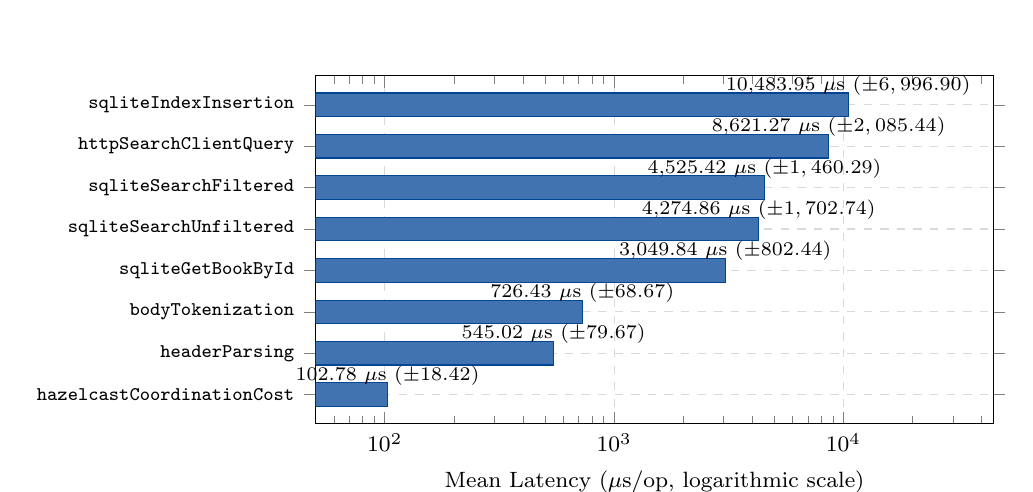
\begin{tikzpicture}
\begin{axis}[
    xbar,
    width=0.84\textwidth,
    height=6.0cm,
    xlabel={Mean Latency ($\mu\text{s/op}$, logarithmic scale)},
    xmode=log,
    xmin=50, xmax=45000,
    symbolic y coords={
        {hazelcastCoordinationCost},
        {headerParsing},
        {bodyTokenization},
        {sqliteGetBookById},
        {sqliteSearchUnfiltered},
        {sqliteSearchFiltered},
        {httpSearchClientQuery},
        {sqliteIndexInsertion}
    },
    ytick=data,
    yticklabel style={font=\scriptsize\ttfamily},
    xlabel style={font=\footnotesize},
    xticklabel style={font=\footnotesize},
    bar width=8.5pt,
    grid=major,
    grid style={dashed,gray!30},
    nodes near coords,
    nodes near coords align={horizontal},
    every node near coord/.append style={font=\scriptsize},
    point meta=explicit symbolic
]
\addplot[fill=ulpgcblue!75, draw=ulpgcblue] coordinates {
    (102.78,{hazelcastCoordinationCost}) [102.78 $\mu$s ($\pm 18.42$)]
    (545.02,{headerParsing}) [545.02 $\mu$s ($\pm 79.67$)]
    (726.43,{bodyTokenization}) [726.43 $\mu$s ($\pm 68.67$)]
    (3049.84,{sqliteGetBookById}) [3,049.84 $\mu$s ($\pm 802.44$)]
    (4274.86,{sqliteSearchUnfiltered}) [4,274.86 $\mu$s ($\pm 1,702.74$)]
    (4525.42,{sqliteSearchFiltered}) [4,525.42 $\mu$s ($\pm 1,460.29$)]
    (8621.27,{httpSearchClientQuery}) [8,621.27 $\mu$s ($\pm 2,085.44$)]
    (10483.95,{sqliteIndexInsertion}) [10,483.95 $\mu$s ($\pm 6,996.90$)]
};
\end{axis}
\end{tikzpicture}
\caption{JMH 1.37 component-level mean latency and $99.9\%$ confidence intervals across indexing and search methods.}
\label{fig:jmh_bars}
\end{figure}

\paragraph{Technical Interpretation of Component Microbenchmarks:}
\begin{enumerate}[leftmargin=*,nosep]
    \item \textbf{Indexing Pipeline Breakdown:} Summed across a single book on native NVMe storage, CPU-bound parsing (\texttt{headerParsing} $= 545.02\,\mu\text{s}$ + \texttt{bodyTokenization} $= 726.43\,\mu\text{s} = 1,271.45\,\mu\text{s}$) accounts for only \textbf{10.7\%} of total indexing time, while Hazelcast coordination (\texttt{hazelcastCoordinationCost} $= 102.78\,\mu\text{s}$) accounts for \textbf{0.87\%}. The remaining \textbf{88.4\%} ($10,483.95\,\mu\text{s} \approx 10.48\text{ ms}$) is spent inside \texttt{SqliteRepository.saveBookIndex()} executing transactional B-tree updates and WAL commits. Notice that \texttt{sqliteIndexInsertion} exhibits higher variance ($\text{StdDev} = 4,628.00\,\mu\text{s}$, ranging from $6,159.22\,\mu\text{s}$ to $17,994.40\,\mu\text{s}$ across the 10 iterations) due to periodic SQLite WAL auto-checkpoints triggered every 1,000 pages.
    \item \textbf{Search Pipeline Breakdown:} Opening a read-only SQLite connection (\texttt{DriverManager.getConnection}) and executing a primary-key lookup (\texttt{sqliteGetBookById}) takes $3.05\text{ ms}$, which establishes the baseline per-query JDBC connection-open cost in \texttt{DatabaseManager}. Executing the inverted-index join \texttt{idx\_postings\_term} + \texttt{COUNT(*) OVER()} + \texttt{ORDER BY p.freq DESC, b.book\_id ASC} adds only $1.22\text{ ms}$ ($4.27\text{ ms}$ total for \texttt{sqliteSearchUnfiltered}), and adding case-insensitive \texttt{author} and \texttt{language} predicates (\texttt{sqliteSearchFiltered}) adds just $0.25\text{ ms}$ ($4.53\text{ ms}$). Traversing the full Javalin/Jetty HTTP stack and Gson serialization (\texttt{httpSearchClientQuery}) adds $4.10\text{ ms}$, yielding $8.62\text{ ms}$ end-to-end in-process latency.
\end{enumerate}

% ==============================================================================
% 6.3 SYSTEM-LEVEL INTEGRATION BENCHMARKS
% ==============================================================================
\subsection{System-Level Integration Benchmarks}
\label{subsec:system_results}

\subsubsection{Per-Book Indexing Latency and Full Atomic Rebuild (\texttt{indexing-book-latency.csv})}
Table~\ref{tab:indexing_latency} reports the live containerized indexing latency measured via \texttt{POST /index/update/\{id\}} across five representative books spanning $37.8\text{ KB}$ to $2,172.7\text{ KB}$, alongside the full 25-book atomic rebuild (\texttt{POST /index/rebuild}).

\begin{table}[!htbp]
\centering
\caption{Live containerized per-book indexing latency (\texttt{POST /index/update/\{id\}}) and full atomic rebuild (\texttt{POST /index/rebuild}) in \texttt{indexing-service} over Docker Desktop WSL2 \texttt{9p} bind-mounted storage (\texttt{./datamarts/metadata.db}). Source: \texttt{indexing-book-latency.csv}.}
\label{tab:indexing_latency}
\scriptsize
\setlength{\tabcolsep}{3.2pt}
\renewcommand{\arraystretch}{1.18}
\begin{tabularx}{\textwidth}{L{3.1cm} L{2.2cm} Y C{1.1cm} R{1.1cm} R{1.1cm} R{1.3cm} R{1.4cm} R{1.0cm} R{1.1cm}}
\toprule
\textbf{Operation (\texttt{indexing})} & \textbf{Backend} & \textbf{Workload (Book ID, Title, Category)} & \textbf{R / T} & \textbf{KB} & \textbf{Postings} & \textbf{Tokens} & \textbf{Lat.\ (ms)} & \textbf{Lat.\ (s)} & \textbf{Post./s} \\
\midrule
\texttt{POST /index/update/1080} & SQLite WAL + HZ & \texttt{1080}: \emph{A Modest Proposal} (Pamphlet) & $2\text{R}/1\text{T}$ & $37.8$ & $1,507$ & $3,991$ & $11,216.60$ & $11.22$ & $134.4$ \\
\texttt{POST /index/update/16}   & SQLite WAL + HZ & \texttt{16}: \emph{Peter Pan} (Medium novel) & $2\text{R}/1\text{T}$ & $281.2$ & $5,090$ & $32,374$ & $25,168.65$ & $25.17$ & $202.2$ \\
\texttt{POST /index/update/1342} & SQLite WAL + HZ & \texttt{1342}: \emph{Pride and Prejudice} (Novel) & $2\text{R}/1\text{T}$ & $753.3$ & $6,864$ & $83,936$ & $31,768.26$ & $31.77$ & $216.1$ \\
\texttt{POST /index/update/2701} & SQLite WAL + HZ & \texttt{2701}: \emph{Moby Dick} (Large EN novel) & $2\text{R}/1\text{T}$ & $1,245.5$ & $16,941$ & $140,870$ & $65,778.74$ & $65.78$ & $257.5$ \\
\texttt{POST /index/update/2000} & SQLite WAL + HZ & \texttt{2000}: \emph{Don Quijote} (Large ES novel) & $2\text{R}/1\text{T}$ & $2,172.7$ & $17,818$ & $227,469$ & $52,602.16$ & $52.60$ & $338.7$ \\
\midrule
\texttt{POST /index/rebuild} & Temp DB $\to$ Swap & All 25 seed books ($15.57\text{ MiB} \to 22.56\text{ MiB}$) & $2\text{R}/4\text{T}$ & $15,922.5$ & $192,167$ & $1,776,589$ & $455,300.00$ & $455.30$ & $422.1$ \\
\bottomrule
\end{tabularx}
\end{table}

\paragraph{Empirical Explanation of Containerized Write Latency:}
Comparing Table~\ref{tab:jmh_results} ($10.48\text{ ms}$ on native Windows NVMe) against Table~\ref{tab:indexing_latency} ($11.22\text{--}65.78\text{ s}$ inside Docker) reveals a critical systems insight:
\begin{itemize}[leftmargin=*,nosep]
    \item \textbf{WSL2 \texttt{9p} Virtual Filesystem Penalty:} Because \path{./datamarts/metadata.db} is bind-mounted from the Windows NTFS host into the Linux container over the Plan 9 (\texttt{9p}/\texttt{drvfs}) protocol, every SQLite page read/write, byte-range file lock (\texttt{fcntl}), and \texttt{fsync} during \texttt{DELETE FROM postings WHERE book\_id = ?} and batched \texttt{INSERT INTO postings} traverses the Hyper-V VM boundary.
    \item \textbf{Dependence on Vocabulary Cardinality (\texttt{COUNT(term)}) and B-Tree Locality:} Both \emph{Moby Dick} (\texttt{2701}, $16,941$ unique terms, $65.78\text{ s}$) and \emph{Don Quijote} (\texttt{2000}, $17,818$ unique terms, $52.60\text{ s}$) insert $\sim 17,000$ rows into \texttt{postings} and update the secondary B-tree \texttt{idx\_postings\_term}. Although \emph{Don Quijote} has a larger body ($2,172.7\text{ KB}$ vs.\ $1,245.5\text{ KB}$), Spanish vocabulary terms cluster into a disjoint lexicographical subspace of \texttt{idx\_postings\_term} (since the other 23 books are English), causing fewer existing B-tree leaf page splits and dirty-page evictions across the \texttt{9p} mount than \emph{Moby Dick}'s 16,941 English terms, which interleave with all 22 other English books.
\end{itemize}

\subsubsection{HTTP Search Throughput and Latency Under Client Concurrency (\texttt{http-search-concurrency.csv})}
Table~\ref{tab:http_concurrency} and Figure~\ref{fig:http_concurrency_plots} present the end-to-end HTTP search performance measured against the Nginx load balancer (\texttt{http://localhost:7000}) routing across $2$ \texttt{search-service} replicas for $c \in \{1, 4, 8, 16, 32\}$.

\begin{table}[!htbp]
\centering
\caption{System-level HTTP search concurrency benchmark against Nginx (\texttt{http://localhost:7000}) balancing $2$ \texttt{search-service} replicas (SQLite WAL Read-Only backend) over the 8-query workload mix. Source: \texttt{docs/benchmarks/http-search-concurrency.csv}.}
\label{tab:http_concurrency}
\scriptsize
\setlength{\tabcolsep}{3.5pt}
\renewcommand{\arraystretch}{1.18}
\begin{tabularx}{\textwidth}{Y C{1.5cm} R{0.8cm} R{0.8cm} R{0.6cm} R{1.4cm} R{1.5cm} R{1.2cm} R{1.3cm} R{1.2cm} R{1.2cm} R{1.2cm}}
\toprule
\textbf{Operation \& Target Stack} & \textbf{Conc.\ / Repl.} & \textbf{Req} & \textbf{OK} & \textbf{Err} & \textbf{Wall (ms)} & \textbf{Thr (req/s)} & \textbf{Mean (ms)} & \textbf{StdDev (ms)} & \textbf{p50 (ms)} & \textbf{p95 (ms)} & \textbf{p99 (ms)} \\
\midrule
\texttt{GET /search} (8-query mix $\to$ Nginx) & $c=1$ / $2\text{R}$ & $25$ & $25$ & $0$ & $1,069.48$ & $23.38$ & $39.65$ & $17.07$ & $43.66$ & $63.35$ & $67.24$ \\
\texttt{GET /search} (8-query mix $\to$ Nginx) & $c=4$ / $2\text{R}$ & $100$ & $100$ & $0$ & $631.36$ & $158.39$ & $23.70$ & $10.69$ & $25.43$ & $39.84$ & $45.62$ \\
\texttt{GET /search} (8-query mix $\to$ Nginx) & $c=8$ / $2\text{R}$ & $200$ & $200$ & $0$ & $517.95$ & $386.14$ & $18.09$ & $12.04$ & $15.94$ & $43.80$ & $52.99$ \\
\texttt{GET /search} (8-query mix $\to$ Nginx) & $c=16$ / $2\text{R}$ & $400$ & $400$ & $0$ & $978.54$ & $408.77$ & $32.22$ & $24.35$ & $25.57$ & $84.79$ & $99.44$ \\
\texttt{GET /search} (8-query mix $\to$ Nginx) & $c=32$ / $2\text{R}$ & $800$ & $800$ & $0$ & $1,730.31$ & $462.35$ & $56.87$ & $46.00$ & $43.85$ & $155.37$ & $182.72$ \\
\bottomrule
\end{tabularx}
\end{table}

\begin{figure}[!htbp]
\centering
\begin{minipage}{0.48\textwidth}
\centering
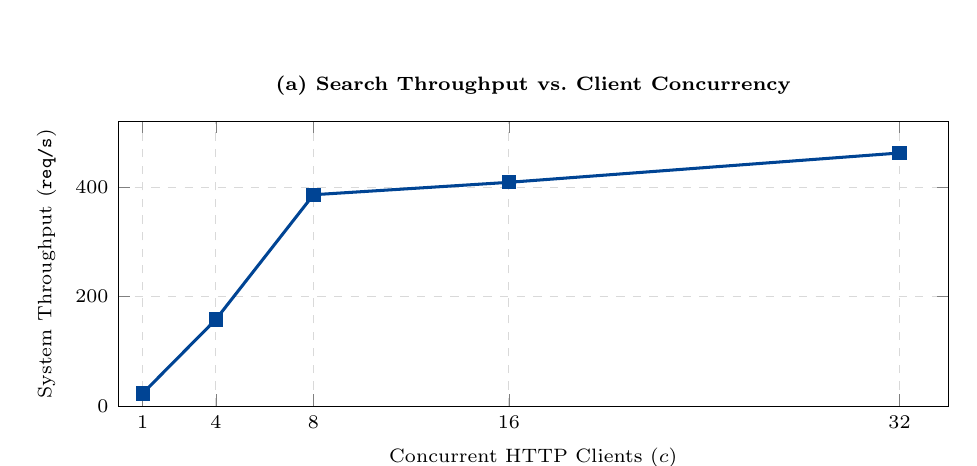
\begin{tikzpicture}
\begin{axis}[
    width=\textwidth,
    height=5.2cm,
    xlabel={Concurrent HTTP Clients ($c$)},
    ylabel={System Throughput (\texttt{req/s})},
    xmin=0, xmax=34,
    ymin=0, ymax=520,
    xtick={1,4,8,16,32},
    grid=major,
    grid style={dashed,gray!30},
    label style={font=\scriptsize},
    tick label style={font=\scriptsize},
    title style={font=\scriptsize\bfseries},
    title={(a) Search Throughput vs.\ Client Concurrency}
]
\addplot[color=ulpgcblue, mark=square*, thick, line width=1.1pt] coordinates {
    (1, 23.38) (4, 158.39) (8, 386.14) (16, 408.77) (32, 462.35)
};
\end{axis}
\end{tikzpicture}
\end{minipage}%
\hfill
\begin{minipage}{0.48\textwidth}
\centering
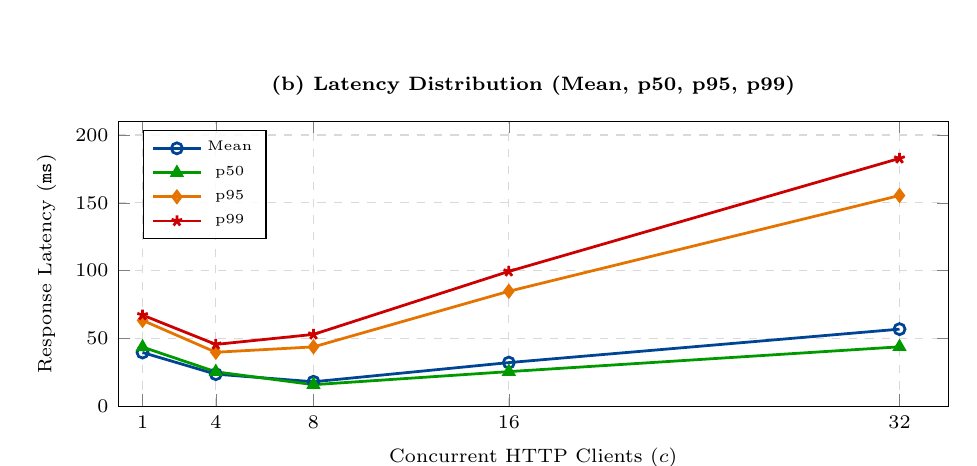
\begin{tikzpicture}
\begin{axis}[
    width=\textwidth,
    height=5.2cm,
    xlabel={Concurrent HTTP Clients ($c$)},
    ylabel={Response Latency (\texttt{ms})},
    xmin=0, xmax=34,
    ymin=0, ymax=210,
    xtick={1,4,8,16,32},
    grid=major,
    grid style={dashed,gray!30},
    label style={font=\scriptsize},
    tick label style={font=\scriptsize},
    legend pos=north west,
    legend style={font=\tiny, fill=white, fill opacity=0.85, draw opacity=1, text opacity=1},
    title style={font=\scriptsize\bfseries},
    title={(b) Latency Distribution (Mean, p50, p95, p99)}
]
\addplot[color=ulpgcblue, mark=o, thick, line width=1.0pt] coordinates {
    (1, 39.65) (4, 23.70) (8, 18.09) (16, 32.22) (32, 56.87)
};
\addlegendentry{Mean}
\addplot[color=green!60!black, mark=triangle*, thick, line width=1.0pt] coordinates {
    (1, 43.66) (4, 25.43) (8, 15.94) (16, 25.57) (32, 43.85)
};
\addlegendentry{p50}
\addplot[color=orange!90!black, mark=diamond*, thick, line width=1.0pt] coordinates {
    (1, 63.35) (4, 39.84) (8, 43.80) (16, 84.79) (32, 155.37)
};
\addlegendentry{p95}
\addplot[color=red!80!black, mark=star, thick, line width=1.0pt] coordinates {
    (1, 67.24) (4, 45.62) (8, 52.99) (16, 99.44) (32, 182.72)
};
\addlegendentry{p99}
\end{axis}
\end{tikzpicture}
\end{minipage}
\caption{Live HTTP search throughput and latency percentiles across concurrency levels $c \in \{1, 4, 8, 16, 32\}$.}
\label{fig:http_concurrency_plots}
\end{figure}

\subsubsection{Container Resource Telemetry and Rigorous Memory Metric Definition (Feedback \#20, \#24, \#29)}
Table~\ref{tab:docker_stats} reports the container telemetry captured in \path{docs/benchmarks/docker-stats.csv} via \texttt{docker stats --no-stream} in Step \texttt{[4/4]} of \path{scripts/run_benchmarks.ps1}, immediately after completing the HTTP search concurrency sweep ($1,525$ requests) and the 5-book live indexing updates, with $2$ \texttt{indexing-service} replicas and $2$ \texttt{search-service} replicas active.

\paragraph{Exact Definition of Memory and Storage Metrics:}
\begin{itemize}[leftmargin=*,nosep]
    \item \textbf{Container Memory Usage (\texttt{MemUsage} in \texttt{docker stats}):} Measures the Linux kernel cgroup v2 resident memory counter (\texttt{memory.current} minus inactive file cache), which includes the JVM Heap, JVM Metaspace, thread stacks, native SQLite JDBC/JNI buffers, and active non-reclaimable kernel buffers inside each container, expressed in binary mebibytes ($\text{MiB} = 2^{20}\text{ bytes}$) relative to the hard cgroup limit (\texttt{deploy.resources.limits.memory}). This is an \emph{observed container working-set measurement}, distinct from the maximum JVM heap allocation flag (\texttt{-Xmx512m} for Java services, \texttt{-Xmx256m} for ActiveMQ). Because the JVM lazily expands its heap up to \texttt{-Xmx} and retains committed heap pages from the OS, \texttt{stage\_2-indexing-1} (which processed the bulk of indexing and rebuild tasks) exhibits a $216.9\text{ MiB}$ resident footprint, whereas \texttt{stage\_2-indexing-2} uses $107.2\text{ MiB}$ and the two stateless \texttt{search-service} replicas consume $129.1\text{ MiB}$ and $127.2\text{ MiB}$ respectively.
    \item \textbf{Aggregate Host Container Footprint:} Across all 8 running containers, total observed resident memory is \textbf{1,038.38 MiB} ($1.014\text{ GiB}$, or $17.67\%$ of the $5,888\text{ MiB}$ sum of container limits and $1.59\%$ of the $64\text{ GB}$ physical host RAM).
\end{itemize}

\begin{table}[!htbp]
\centering
\caption{Measured container resource telemetry (\texttt{docker stats --no-stream}) captured post-benchmark with 8 active containers ($2$ \texttt{indexing} replicas, $2$ \texttt{search} replicas). Source: \texttt{docs/benchmarks/docker-stats.csv}.}
\label{tab:docker_stats}
\scriptsize
\setlength{\tabcolsep}{3.5pt}
\renewcommand{\arraystretch}{1.18}
\begin{tabularx}{\textwidth}{L{2.8cm} Y C{1.5cm} R{1.1cm} R{2.9cm} R{1.1cm} R{2.4cm} R{2.2cm}}
\toprule
\textbf{Container Instance} & \textbf{Service Role} & \textbf{JVM \texttt{-Xmx}} & \textbf{CPU (\%)} & \textbf{Working Set / Limit} & \textbf{Mem (\%)} & \textbf{Net I/O (RX / TX)} & \textbf{Block I/O (R / W)} \\
\midrule
\texttt{stage\_2-nginx-1}     & Reverse Proxy Gateway & N/A (C) & $0.00\%$ & $4.438\text{ MiB} / 128\text{ MiB}$ & $3.47\%$  & $1.67\text{ MB} / 1.84\text{ MB}$ & $0\text{ B} / 12.3\text{ kB}$ \\
\texttt{stage\_2-search-1}    & Search Replica 1 (RO) & \texttt{512m} & $0.54\%$ & $129.1\text{ MiB} / 768\text{ MiB}$ & $16.81\%$ & $485\text{ kB} / 1.58\text{ MB}$  & $0\text{ B} / 1.69\text{ MB}$ \\
\texttt{stage\_2-search-2}    & Search Replica 2 (RO) & \texttt{512m} & $0.54\%$ & $127.2\text{ MiB} / 768\text{ MiB}$ & $16.56\%$ & $487\text{ kB} / 1.54\text{ MB}$  & $0\text{ B} / 1.70\text{ MB}$ \\
\texttt{stage\_2-indexing-1}  & Indexing Replica 1    & \texttt{512m} & $3.12\%$ & $216.9\text{ MiB} / 1\text{ GiB}$   & $21.18\%$ & $261\text{ kB} / 917\text{ kB}$   & $0\text{ B} / 25.2\text{ MB}$ \\
\texttt{stage\_2-indexing-2}  & Indexing Replica 2    & \texttt{512m} & $3.66\%$ & $107.2\text{ MiB} / 1\text{ GiB}$   & $10.47\%$ & $68.5\text{ kB} / 294\text{ kB}$  & $0\text{ B} / 1.31\text{ MB}$ \\
\texttt{stage\_2-ingestion-1} & Ingestion Service     & \texttt{512m} & $0.57\%$ & $92.84\text{ MiB} / 768\text{ MiB}$ & $12.09\%$ & $68.1\text{ kB} / 299\text{ kB}$  & $0\text{ B} / 291\text{ kB}$ \\
\texttt{stage\_2-activemq-1}  & ActiveMQ JMS Broker   & \texttt{256m} & $0.24\%$ & $178.4\text{ MiB} / 512\text{ MiB}$ & $34.85\%$ & $112\text{ kB} / 72\text{ kB}$    & $0\text{ B} / 901\text{ kB}$ \\
\texttt{stage\_2-hazelcast-1} & Hazelcast Instance    & Default       & $0.98\%$ & $182.3\text{ MiB} / 512\text{ MiB}$ & $35.60\%$ & $3.64\text{ MB} / 905\text{ kB}$  & $0\text{ B} / 918\text{ kB}$ \\
\midrule
\multicolumn{3}{l}{\textbf{Aggregate Stack Totals (8 Containers on Single Host)}} & \textbf{9.65\%} & \textbf{1,038.38 / 5,888 MiB} & \textbf{17.67\%} & \textbf{6.79 MB / 7.45 MB} & \textbf{0 B / 32.02 MB} \\
\bottomrule
\end{tabularx}
\end{table}

% ==============================================================================
% 6.4 REPLICATION, THREADING & BOTTLENECK ANALYSIS
% ==============================================================================
\subsection{Replication, Threading, and Bottleneck Analysis}
\label{subsec:bottleneck_analysis}

\begin{enumerate}[leftmargin=*,nosep]
    \item \textbf{Read Path Scalability and the Knee of the Curve ($c = 8$ vs.\ $c = 32$):}
    In Table~\ref{tab:http_concurrency}, Nginx distributes incoming requests evenly across \texttt{stage\_2-search-1} ($485\text{ kB}$ RX / $1.58\text{ MB}$ TX) and \texttt{stage\_2-search-2} ($487\text{ kB}$ RX / $1.54\text{ MB}$ TX). Moving from $c=1$ to $c=8$ reduces mean latency from $39.65\text{ ms}$ to $18.09\text{ ms}$ ($p_{50} = 15.94\text{ ms}$) while increasing throughput $16.5\times$ ($23.38 \to 386.14\text{ req/s}$), because concurrent PowerShell runspaces amortize client-side scheduling overhead and keep both search replicas' $1.0\text{-vCPU}$ allocations busy without queuing. Beyond $c=8$, the two search replicas reach their Docker CPU quota ($2 \times 1.0 = 2.0\text{ vCPUs}$ total) and open a fresh read-only SQLite connection per request (\texttt{DatabaseManager.getConnection()}, which costs $3.05\text{ ms}$ per call in JMH). Consequently, from $c=8$ to $c=32$, throughput plateaus near \textbf{462.35 req/s} ($+19.7\%$) while Little's Law ($L = \lambda W$) manifests as rising queuing latency: mean latency grows $3.14\times$ ($18.09 \to 56.87\text{ ms}$) and $p_{95}$ grows $3.55\times$ ($43.80 \to 155.37\text{ ms}$).
    \item \textbf{Write Path Bottleneck (Parallel Parsing vs.\ Serialized SQLite Commits):}
    During indexing and full rebuilds, \texttt{HeaderParser} and \texttt{BodyTokenizer} scale across \texttt{JMS\_CONSUMERS=2}, \texttt{INDEXING\_REPLICAS=2}, and \texttt{INDEX\_WORKER\_THREADS=4}. However, because parsing takes only $1.27\text{ ms/book}$ while SQLite persistence takes $10.48\text{ ms/book}$ on native NVMe and $11.22\text{--}65.78\text{ s/book}$ over the WSL2 \texttt{9p} bind mount, Amdahl's Law dictates that the serialized critical section guarded by \texttt{FencedLock("index-writer")} is the dominant write bottleneck. In \texttt{IndexRebuilder.indexInto()}, worker threads parse batches of $8$ books concurrently via \texttt{executor.submit()}, but \texttt{target.saveBookIndex()} is invoked sequentially per book, and every \texttt{saveBookIndex()} opens a new JDBC connection and executes a full \texttt{conn.commit()} (\texttt{fsync}).
\end{enumerate}

% ==============================================================================
% 6.5 LIMITATIONS AND THREATS TO VALIDITY
% ==============================================================================
\subsection{Limitations and Threats to Validity (Feedback \#12, \#13, \#31, \#34)}
\label{subsec:limitations}

To ensure strict academic and engineering rigor, we explicitly state the scope boundaries and threats to validity of our Stage 2 experimental evaluation:
\begin{enumerate}[leftmargin=*,nosep]
    \item \textbf{Single-Host Deployment Scope (No Extrapolation to Multi-Node Clusters):} All eight containers (\texttt{nginx}, $2\times\texttt{search}$, $2\times\texttt{indexing}$, \texttt{ingestion}, \texttt{activemq}, \texttt{hazelcast}) and the client load generator ran on a \textbf{single physical machine} sharing the same CPU, memory bus, kernel loopback network, and NVMe SSD. Therefore, these results validate cooperative SOA decoupling and concurrency on a single host, and \textbf{must not be extrapolated} as proof of horizontal scalability across a multi-node distributed cluster (where inter-node NIC latency, network partitioning, and distributed storage replication come into play).
    \item \textbf{Corpus Size Scope ($N = 25$ Books, $15.57\text{ MiB}$ Text, $22.60\text{ MiB}$ SQLite Index):} The entire $22.60\text{ MiB}$ SQLite database ($5,785$ pages) fits comfortably inside the OS page cache ($31.05\text{ GiB}$ WSL2 RAM). For a corpus of $100,000+$ books where the inverted index exceeds physical RAM, read queries would incur physical disk read I/O and \texttt{COUNT(*) OVER()} window scans on high-frequency terms would require index-only count pre-aggregation.
    \item \textbf{WSL2 \texttt{9p} Bind-Mount Distortion on Containerized SQLite Writes:} Mounting Windows NTFS directories (\path{./datalake}, \path{./datamarts}) into Linux containers via WSL2 \texttt{9p} inflates SQLite transaction commit times by three orders of magnitude ($10.48\text{ ms}$ native NVMe vs.\ $11.22\text{--}65.78\text{ s}$ in container). While this does not affect read-only search queries once cached in memory ($18.09\text{ ms}$ at $c=8$), it heavily dominates containerized indexing wall time.
    \item \textbf{Per-Query JDBC Connection Opening in \texttt{DatabaseManager}:} \texttt{DatabaseManager.getConnection()} opens and closes a read-only SQLite JDBC connection on every query rather than using a persistent connection pool (e.g., HikariCP). As shown in Table~\ref{tab:jmh_results}, connection initialization accounts for $\sim 3.05\text{ ms}$ of the $4.27\text{ ms}$ query latency.
    \item \textbf{Single-Member Hazelcast CP Configuration:} In \path{hazelcast/hazelcast.yaml}, \texttt{cp-member-count: 1} and \texttt{group-size: 1} are used because Stage 2 deploys a single Hazelcast Instance container. Real Raft consensus fault tolerance requires at least $3$ Hazelcast members.
\end{enumerate}

% ==============================================================================
% SECTION 7: CONCLUSIONS AND STAGE 3 PREPARATION
% ==============================================================================
\section{Conclusions and Stage 3 Preparation}
\label{sec:conclusions}

\subsection{Empirical Conclusions Scoped to the Stage 2 Single-Host Deployment}
Based strictly on the empirical measurements and automated test evidence collected on our 25-book multilingual corpus ($15.57\text{ MiB}$ logical datalake size across $100$ files, $192,167$ inverted-index postings in a $22.60\text{ MiB}$ SQLite WAL datamart) deployed on a single host, we conclude:
\begin{enumerate}[leftmargin=*,nosep]
    \item \textbf{Effective Decoupling and Crash Consistency:} Decomposing the Stage 1 monolith into \texttt{ingestion-service}, \texttt{indexing-service}, and \texttt{search-service} connected via ActiveMQ queues and Hazelcast Client-to-Instance coordination eliminates synchronous ingestion blocking and isolates failure domains. Our 41-test JUnit suite and live fault-injection checks confirm that the dual Transactional Outbox (\texttt{OutboxService} and \texttt{BookIndexedPublisher}), lease-based \texttt{BookClaim} takeover, and transactional SQLite rollback guarantee at-least-once event delivery and prevent any failed parse or database write from ever marking a book as \texttt{INDEXED}.
    \item \textbf{Zero-Downtime Index Rebuilding:} Building replacement indexes in an isolated temporary database (\path{metadata.db.rebuild-<uuid>.tmp}) under \texttt{FencedLock("lock:index-rebuild")} and swapping tables atomically via \texttt{ATTACH DATABASE} under \texttt{FencedLock("index-writer")} allows \texttt{search-service} replicas to serve continuous \texttt{HTTP 200 OK} responses (\texttt{total=13} for \texttt{q=adventure}) throughout the entire $455.30\text{ s}$ rebuild while rejecting overlapping rebuilds in $<15\text{ ms}$ with \texttt{HTTP 409 Conflict}.
    \item \textbf{Quantified Single-Host Performance Envelope:} On native storage (JMH), header parsing ($545.02\,\mu\text{s}$), body tokenization ($726.43\,\mu\text{s}$), and Hazelcast coordination ($102.78\,\mu\text{s}$) are sub-millisecond, whereas SQLite persistence ($10,483.95\,\mu\text{s}$) accounts for $88.4\%$ of indexing cost. Under concurrent HTTP load across $2$ \texttt{search-service} replicas behind Nginx, the system achieves its optimal latency-throughput balance at $c=8$ ($386.14\text{ req/s}$, mean latency $18.09\text{ ms}$, $p_{95} = 43.80\text{ ms}$) and reaches a peak throughput of \textbf{462.35 req/s} at $c=32$ ($0\%$ errors across $1,525$ requests) within a total 8-container memory footprint of $1,038.38\text{ MiB}$.
\end{enumerate}

\subsection{Architectural Roadmap for Stage 3 (Multi-Node Cluster Deployment)}
Transitioning from a single-host Docker Compose environment to a multi-node distributed cluster in \textbf{Stage 3} invalidates several local assumptions. Table~\ref{tab:stage3_roadmap} details the concrete architectural changes required across storage, coordination, messaging, and networking.

\begin{table}[!htbp]
\centering
\caption{Architectural migration roadmap from Stage 2 (Single-Host SOA) to Stage 3 (Multi-Node Cluster Deployment).}
\label{tab:stage3_roadmap}
\scriptsize
\setlength{\tabcolsep}{4pt}
\renewcommand{\arraystretch}{1.18}
\begin{tabularx}{\textwidth}{L{3.0cm} L{5.0cm} Y}
\toprule
\textbf{Architectural Area} & \textbf{Stage 2 Single-Host Assumption} & \textbf{Stage 3 Multi-Node Cluster Evolution} \\
\midrule
\textbf{1. Datalake Storage} & Local bind mount (\path{./datalake:/data/datalake}) shared between \texttt{ingestion} and \texttt{indexing} on the same host OS. & Replace local filesystem bind mounts with an S3-compatible distributed object store (e.g., \textbf{MinIO} or Ceph) or replicated HDFS, storing immutable header/body objects and metadata tags accessible from any cluster node. \\
\addlinespace[2pt]
\textbf{2. Datamart \& SQLite WAL Limitation} & Single \path{./datamarts/metadata.db} file shared by writer and readers via host kernel page cache and POSIX \path{metadata.db-shm} shared memory. & SQLite WAL \texttt{-shm} shared memory cannot operate safely across network filesystems (NFS/SMB). In Stage 3, either (a) ship immutable versioned SQLite snapshots (\texttt{metadata\_v<N>.db}) to local NVMe disks on each \texttt{search-service} node upon receiving \texttt{BookIndexed} events, or (b) migrate the inverted index to a distributed/sharded store (e.g., PostgreSQL/Citus or Hazelcast partitioned \texttt{IMap}s). \\
\addlinespace[2pt]
\textbf{3. Write Bottleneck \& Sharding} & Global single-writer serialization via \texttt{FencedLock("index-writer")} and per-book \texttt{fsync} over WSL2 \texttt{9p}. & Partition the index by \texttt{book\_id} or term hash across $K$ independent shards with per-shard locks, use native Linux ext4/XFS volumes instead of \texttt{9p} bind mounts, and pool JDBC connections (HikariCP). \\
\addlinespace[2pt]
\textbf{4. Hazelcast Instances, Partitioning \& Backups} & Single Hazelcast \textbf{Instance} container (\texttt{cp-member-count: 1}, \texttt{group-size: 1}) with 271 partitions on 1 node and no backup replicas if the node crashes. & Deploy $\ge 3$ Hazelcast \textbf{Instances (Cluster Members)} across physical hosts with \texttt{setBackupCount(2)} (1 primary + 2 backup replicas across the 271 partitions) and \texttt{cp-member-count: 3} (Raft quorum), while microservices connect via \texttt{HazelcastClient}. \\
\addlinespace[2pt]
\textbf{5. ActiveMQ Broker High Availability} & Single ActiveMQ instance (\texttt{tcp://activemq:61616}) acting as a single point of failure for event queuing. & Deploy an ActiveMQ Primary/Secondary shared-storage cluster or Network of Brokers and configure clients with \path{failover:(tcp://broker1:61616,tcp://broker2:61616)?randomize=false}. \\
\addlinespace[2pt]
\textbf{6. Network Discovery \& Partitions} & Static Docker Compose bridge DNS (\texttt{hazelcast:5701}, \texttt{search:7000}) on a reliable local virtual switch. & Deploy over a multi-host overlay network (Docker Swarm or Kubernetes) with TCP-IP/Kubernetes member discovery (\texttt{TcpIpConfig.addMember(...)}) in \path{hazelcast.yaml}, health-aware ingress load balancing, and split-brain protection. \\
\bottomrule
\end{tabularx}
\end{table}

% ==============================================================================
% SECTION 8: REFERENCES (MANDATORY RULE #2 - ZERO BROKEN CITATIONS)
% ==============================================================================
\begin{thebibliography}{99}

\bibitem{ulpgc_stage2_spec}
Universidad de Las Palmas de Gran Canaria (ULPGC), Escuela de Ingenier\'ia Inform\'atica,
\emph{Big Data Course Project --- Stage 2: Building a Service-Oriented Architecture (SOA) Specification and Evaluation Rubric},
Grado en Ciencia e Ingenier\'ia de Datos, Academic Year 2025--2026.

\bibitem{ulpgc_stage1_spec}
Universidad de Las Palmas de Gran Canaria (ULPGC), Escuela de Ingenier\'ia Inform\'atica,
\emph{Big Data Course Project --- Stage 1: Monolithic Search Engine Prototype and Evaluation Feedback},
Grado en Ciencia e Ingenier\'ia de Datos, Academic Year 2025--2026.

\bibitem{fourbytees_benchmarks}
Group FourByTees (\texttt{com.fourbytees}: L.~Rodr\'iguez Hern\'andez, J.~Bol\'ivar Garc\'ia, J.~Argoitia, and S.~D\'evora Ortega),
\emph{Stage 2 Reproducible Benchmark Dataset and Automation Suite (\texttt{scripts/run\_benchmarks.ps1}, \texttt{docs/benchmarks/*.csv/.json}, commit \texttt{5c4ee06})},
GitHub Repository: \url{https://github.com/4Bytees/stage_2}, Nov.\ 2026.

\bibitem{javalin_docs}
Javalin Project,
\emph{Javalin 6.1.3 Documentation --- Lightweight Java and Kotlin Web Framework on Eclipse Jetty},
2024. [Online]. Available: \url{https://javalin.io/documentation}

\bibitem{hazelcast_docs}
Hazelcast, Inc.\ and ULPGC Big Data Course Notes,
\emph{Hazelcast Platform 5.3.6 Reference Manual --- Cluster Construction (Instances vs.\ Clients), Distributed Data Structures (\texttt{IMap}), Replication/Partitioning, and CP Subsystem},
2024. [Online]. Available: \url{https://docs.hazelcast.com/hazelcast/5.3/}

\bibitem{activemq_docs}
Apache Software Foundation,
\emph{Apache ActiveMQ Classic 5.18.3 Documentation --- Persistent JMS Queues, Redelivery Policy, and Dead-Letter Queues},
2024. [Online]. Available: \url{https://activemq.apache.org/components/classic/documentation}

\bibitem{sqlite_wal_docs}
SQLite Consortium,
\emph{Write-Ahead Logging (WAL Mode) and File Locking Concurrency in SQLite 3.45},
2024. [Online]. Available: \url{https://www.sqlite.org/wal.html}

\bibitem{jmh_docs}
OpenJDK Project,
\emph{Java Microbenchmark Harness (JMH) v1.37 Documentation and Annotation Processor Reference},
2024. [Online]. Available: \url{https://github.com/openjdk/jmh}

\bibitem{docker_docs}
Docker, Inc.\ and ULPGC Big Data Course Notes,
\emph{Docker Containerization Platform, Engine 29.9, and Docker Compose v5 Specification --- Images, Containers, Resource Constraints, and WSL2 Storage Backend},
2026. [Online]. Available: \url{https://docs.docker.com/reference/compose-file/}

\bibitem{nginx_docs}
F5, Inc.,
\emph{NGINX HTTP Load Balancing and Reverse Proxy Configuration (\texttt{ngx\_http\_upstream\_module})},
2024. [Online]. Available: \url{https://nginx.org/en/docs/http/load_balancing.html}

\bibitem{openapi_spec}
OpenAPI Initiative (Linux Foundation),
\emph{OpenAPI Specification v3.0.3},
2020. [Online]. Available: \url{https://spec.openapis.org/oas/v3.0.3}

\bibitem{gutenberg_docs}
Project Gutenberg Literary Archive Foundation,
\emph{Project Gutenberg eBook Mirror and Plain-Text Header Conventions},
2024. [Online]. Available: \url{https://www.gutenberg.org/}

\bibitem{microservices_richardson}
C.~Richardson,
\emph{Microservices Patterns: With Examples in Java} (Transactional Outbox, Competing Consumers, and Saga Choreography Patterns),
Shelter Island, NY, USA: Manning Publications, 2018.

\bibitem{kleppmann_ddia}
M.~Kleppmann,
\emph{Designing Data-Intensive Applications: The Big Ideas Behind Reliable, Scalable, and Maintainable Systems},
Sebastopol, CA, USA: O'Reilly Media, 2017.

\end{thebibliography}

\end{document}
